\documentclass[twoside]{book}

% Packages required by doxygen
\usepackage{fixltx2e}
\usepackage{calc}
\usepackage{doxygen}
\usepackage[export]{adjustbox} % also loads graphicx
\usepackage{graphicx}
\usepackage[utf8]{inputenc}
\usepackage{makeidx}
\usepackage{multicol}
\usepackage{multirow}
\PassOptionsToPackage{warn}{textcomp}
\usepackage{textcomp}
\usepackage[nointegrals]{wasysym}
\usepackage[table]{xcolor}

% Font selection
\usepackage[T1]{fontenc}
\usepackage[scaled=.90]{helvet}
\usepackage{courier}
\usepackage{amssymb}
\usepackage{sectsty}
\renewcommand{\familydefault}{\sfdefault}
\allsectionsfont{%
  \fontseries{bc}\selectfont%
  \color{darkgray}%
}
\renewcommand{\DoxyLabelFont}{%
  \fontseries{bc}\selectfont%
  \color{darkgray}%
}
\newcommand{\+}{\discretionary{\mbox{\scriptsize$\hookleftarrow$}}{}{}}

% Page & text layout
\usepackage{geometry}
\geometry{%
  a4paper,%
  top=2.5cm,%
  bottom=2.5cm,%
  left=2.5cm,%
  right=2.5cm%
}
\tolerance=750
\hfuzz=15pt
\hbadness=750
\setlength{\emergencystretch}{15pt}
\setlength{\parindent}{0cm}
\setlength{\parskip}{3ex plus 2ex minus 2ex}
\makeatletter
\renewcommand{\paragraph}{%
  \@startsection{paragraph}{4}{0ex}{-1.0ex}{1.0ex}{%
    \normalfont\normalsize\bfseries\SS@parafont%
  }%
}
\renewcommand{\subparagraph}{%
  \@startsection{subparagraph}{5}{0ex}{-1.0ex}{1.0ex}{%
    \normalfont\normalsize\bfseries\SS@subparafont%
  }%
}
\makeatother

% Headers & footers
\usepackage{fancyhdr}
\pagestyle{fancyplain}
\fancyhead[LE]{\fancyplain{}{\bfseries\thepage}}
\fancyhead[CE]{\fancyplain{}{}}
\fancyhead[RE]{\fancyplain{}{\bfseries\leftmark}}
\fancyhead[LO]{\fancyplain{}{\bfseries\rightmark}}
\fancyhead[CO]{\fancyplain{}{}}
\fancyhead[RO]{\fancyplain{}{\bfseries\thepage}}
\fancyfoot[LE]{\fancyplain{}{}}
\fancyfoot[CE]{\fancyplain{}{}}
\fancyfoot[RE]{\fancyplain{}{\bfseries\scriptsize Generated by Doxygen }}
\fancyfoot[LO]{\fancyplain{}{\bfseries\scriptsize Generated by Doxygen }}
\fancyfoot[CO]{\fancyplain{}{}}
\fancyfoot[RO]{\fancyplain{}{}}
\renewcommand{\footrulewidth}{0.4pt}
\renewcommand{\chaptermark}[1]{%
  \markboth{#1}{}%
}
\renewcommand{\sectionmark}[1]{%
  \markright{\thesection\ #1}%
}

% Indices & bibliography
\usepackage{natbib}
\usepackage[titles]{tocloft}
\setcounter{tocdepth}{3}
\setcounter{secnumdepth}{5}
\makeindex

% Hyperlinks (required, but should be loaded last)
\usepackage{ifpdf}
\ifpdf
  \usepackage[pdftex,pagebackref=true]{hyperref}
\else
  \usepackage[ps2pdf,pagebackref=true]{hyperref}
\fi
\hypersetup{%
  colorlinks=true,%
  linkcolor=blue,%
  citecolor=blue,%
  unicode%
}

% Custom commands
\newcommand{\clearemptydoublepage}{%
  \newpage{\pagestyle{empty}\cleardoublepage}%
}

\usepackage{caption}
\captionsetup{labelsep=space,justification=centering,font={bf},singlelinecheck=off,skip=4pt,position=top}

%===== C O N T E N T S =====

\begin{document}

% Titlepage & ToC
\hypersetup{pageanchor=false,
             bookmarksnumbered=true,
             pdfencoding=unicode
            }
\pagenumbering{alph}
\begin{titlepage}
\vspace*{7cm}
\begin{center}%
{\Large College Tour Project }\\
\vspace*{1cm}
{\large Generated by Doxygen 1.8.14}\\
\end{center}
\end{titlepage}
\clearemptydoublepage
\pagenumbering{roman}
\tableofcontents
\clearemptydoublepage
\pagenumbering{arabic}
\hypersetup{pageanchor=true}

%--- Begin generated contents ---
\chapter{College\+Tour}
\label{md__r_e_a_d_m_e}
\Hypertarget{md__r_e_a_d_m_e}
\input{md__r_e_a_d_m_e}
\chapter{Namespace Index}
\section{Namespace List}
Here is a list of all documented namespaces with brief descriptions\+:\begin{DoxyCompactList}
\item\contentsline{section}{\mbox{\hyperlink{namespace_ui}{Ui}} }{\pageref{namespace_ui}}{}
\end{DoxyCompactList}

\chapter{Hierarchical Index}
\section{Class Hierarchy}
This inheritance list is sorted roughly, but not completely, alphabetically\+:\begin{DoxyCompactList}
\item \contentsline{section}{Cart}{\pageref{class_cart}}{}
\item \contentsline{section}{College}{\pageref{struct_college}}{}
\item \contentsline{section}{db\+Manager}{\pageref{classdb_manager}}{}
\item \contentsline{section}{Distance}{\pageref{struct_distance}}{}
\item Q\+Dialog\begin{DoxyCompactList}
\item \contentsline{section}{totals\+Sheet}{\pageref{classtotals_sheet}}{}
\end{DoxyCompactList}
\item Q\+Main\+Window\begin{DoxyCompactList}
\item \contentsline{section}{Main\+Window}{\pageref{class_main_window}}{}
\end{DoxyCompactList}
\item Q\+Widget\begin{DoxyCompactList}
\item \contentsline{section}{College\+Model}{\pageref{class_college_model}}{}
\item \contentsline{section}{maintenance}{\pageref{classmaintenance}}{}
\end{DoxyCompactList}
\item \contentsline{section}{souvenir\+Item}{\pageref{structsouvenir_item}}{}
\item \contentsline{section}{Transaction}{\pageref{class_transaction}}{}
\item \contentsline{section}{Ui\+\_\+\+College\+Model}{\pageref{class_ui___college_model}}{}
\begin{DoxyCompactList}
\item \contentsline{section}{Ui\+:\+:College\+Model}{\pageref{class_ui_1_1_college_model}}{}
\end{DoxyCompactList}
\item \contentsline{section}{Ui\+\_\+maintenance}{\pageref{class_ui__maintenance}}{}
\begin{DoxyCompactList}
\item \contentsline{section}{Ui\+:\+:maintenance}{\pageref{class_ui_1_1maintenance}}{}
\end{DoxyCompactList}
\item \contentsline{section}{Ui\+\_\+\+Main\+Window}{\pageref{class_ui___main_window}}{}
\begin{DoxyCompactList}
\item \contentsline{section}{Ui\+:\+:Main\+Window}{\pageref{class_ui_1_1_main_window}}{}
\end{DoxyCompactList}
\item \contentsline{section}{Ui\+\_\+totals}{\pageref{class_ui__totals}}{}
\begin{DoxyCompactList}
\item \contentsline{section}{Ui\+:\+:totals}{\pageref{class_ui_1_1totals}}{}
\end{DoxyCompactList}
\item \contentsline{section}{Ui\+\_\+totals\+Sheet}{\pageref{class_ui__totals_sheet}}{}
\begin{DoxyCompactList}
\item \contentsline{section}{Ui\+:\+:totals\+Sheet}{\pageref{class_ui_1_1totals_sheet}}{}
\end{DoxyCompactList}
\end{DoxyCompactList}

\chapter{Class Index}
\section{Class List}
Here are the classes, structs, unions and interfaces with brief descriptions\+:\begin{DoxyCompactList}
\item\contentsline{section}{\mbox{\hyperlink{class_cart}{Cart}} \\*The \mbox{\hyperlink{class_cart}{Cart}} class }{\pageref{class_cart}}{}
\item\contentsline{section}{\mbox{\hyperlink{struct_college}{College}} \\*The \mbox{\hyperlink{struct_college}{College}} struct Stores colleges with their relevant data as well as operations to compare to other college structs }{\pageref{struct_college}}{}
\item\contentsline{section}{\mbox{\hyperlink{class_ui_1_1_college_model}{Ui\+::\+College\+Model}} }{\pageref{class_ui_1_1_college_model}}{}
\item\contentsline{section}{\mbox{\hyperlink{class_college_model}{College\+Model}} \\*The \mbox{\hyperlink{class_college_model}{College\+Model}} class The class that will process all the functionality of the UI and allow the user to properly plan their trip and make purchases }{\pageref{class_college_model}}{}
\item\contentsline{section}{\mbox{\hyperlink{classdb_manager}{db\+Manager}} \\*The \mbox{\hyperlink{classdb_manager}{db\+Manager}} class Class to handle all functionality of a S\+Q\+Lite database. Allows only a single instance to be created and uses that instance throughout execution. All data will be represented in Q\+Vectors and queries }{\pageref{classdb_manager}}{}
\item\contentsline{section}{\mbox{\hyperlink{struct_distance}{Distance}} \\*The \mbox{\hyperlink{struct_distance}{Distance}} struct Stores distances between two colleges }{\pageref{struct_distance}}{}
\item\contentsline{section}{\mbox{\hyperlink{classmaintenance}{maintenance}} \\*The maintenance class This class will handle basic operations of User-\/\+Interface and altering database records used in the program }{\pageref{classmaintenance}}{}
\item\contentsline{section}{\mbox{\hyperlink{class_ui_1_1maintenance}{Ui\+::maintenance}} }{\pageref{class_ui_1_1maintenance}}{}
\item\contentsline{section}{\mbox{\hyperlink{class_ui_1_1_main_window}{Ui\+::\+Main\+Window}} }{\pageref{class_ui_1_1_main_window}}{}
\item\contentsline{section}{\mbox{\hyperlink{class_main_window}{Main\+Window}} }{\pageref{class_main_window}}{}
\item\contentsline{section}{\mbox{\hyperlink{structsouvenir_item}{souvenir\+Item}} \\*The \mbox{\hyperlink{structsouvenir_item}{souvenir\+Item}} struct Will replicate details of a souvenir and will be composed into colleges to represent their souvenirs }{\pageref{structsouvenir_item}}{}
\item\contentsline{section}{\mbox{\hyperlink{class_ui_1_1totals}{Ui\+::totals}} }{\pageref{class_ui_1_1totals}}{}
\item\contentsline{section}{\mbox{\hyperlink{class_ui_1_1totals_sheet}{Ui\+::totals\+Sheet}} }{\pageref{class_ui_1_1totals_sheet}}{}
\item\contentsline{section}{\mbox{\hyperlink{classtotals_sheet}{totals\+Sheet}} \\*The \mbox{\hyperlink{classtotals_sheet}{totals\+Sheet}} class UI to display the expenses and invoice from the trip at the time it was invoked }{\pageref{classtotals_sheet}}{}
\item\contentsline{section}{\mbox{\hyperlink{class_transaction}{Transaction}} \\*The \mbox{\hyperlink{class_transaction}{Transaction}} class }{\pageref{class_transaction}}{}
\item\contentsline{section}{\mbox{\hyperlink{class_ui___college_model}{Ui\+\_\+\+College\+Model}} }{\pageref{class_ui___college_model}}{}
\item\contentsline{section}{\mbox{\hyperlink{class_ui__maintenance}{Ui\+\_\+maintenance}} }{\pageref{class_ui__maintenance}}{}
\item\contentsline{section}{\mbox{\hyperlink{class_ui___main_window}{Ui\+\_\+\+Main\+Window}} }{\pageref{class_ui___main_window}}{}
\item\contentsline{section}{\mbox{\hyperlink{class_ui__totals}{Ui\+\_\+totals}} }{\pageref{class_ui__totals}}{}
\item\contentsline{section}{\mbox{\hyperlink{class_ui__totals_sheet}{Ui\+\_\+totals\+Sheet}} }{\pageref{class_ui__totals_sheet}}{}
\end{DoxyCompactList}

\chapter{Namespace Documentation}
\hypertarget{namespace_ui}{}\section{Ui Namespace Reference}
\label{namespace_ui}\index{Ui@{Ui}}
\subsection*{Classes}
\begin{DoxyCompactItemize}
\item 
class \mbox{\hyperlink{class_ui_1_1_college_model}{College\+Model}}
\item 
class \mbox{\hyperlink{class_ui_1_1maintenance}{maintenance}}
\item 
class \mbox{\hyperlink{class_ui_1_1_main_window}{Main\+Window}}
\item 
class \mbox{\hyperlink{class_ui_1_1totals}{totals}}
\item 
class \mbox{\hyperlink{class_ui_1_1totals_sheet}{totals\+Sheet}}
\end{DoxyCompactItemize}


\subsection{Detailed Description}
\mbox{\hyperlink{struct_college}{College}} Model Interface This class will handle the functionality the user will interact with. Public functions will allow most program capabilities and the private data will be processed and stored. The UI class will allow a student to generate a college trip and the ability to purchase souvenirs along the way. 
\chapter{Class Documentation}
\hypertarget{class_cart}{}\section{Cart Class Reference}
\label{class_cart}\index{Cart@{Cart}}


The \mbox{\hyperlink{class_cart}{Cart}} class.  




{\ttfamily \#include $<$cart.\+h$>$}

\subsection*{Public Member Functions}
\begin{DoxyCompactItemize}
\item 
\mbox{\Hypertarget{class_cart_a596ee7e7ced21478d39b6afe67828a2b}\label{class_cart_a596ee7e7ced21478d39b6afe67828a2b}} 
\mbox{\hyperlink{class_cart_a596ee7e7ced21478d39b6afe67828a2b}{Cart}} ()
\begin{DoxyCompactList}\small\item\em Default Constructor. \end{DoxyCompactList}\item 
int \mbox{\hyperlink{class_cart_ac89333c3766ab987cad13fc430407b78}{size}} ()
\begin{DoxyCompactList}\small\item\em Function to return size of transactions vector. \end{DoxyCompactList}\item 
void \mbox{\hyperlink{class_cart_aa85e6745516afcd9b46fac6397aa5439}{print\+Cart}} ()
\begin{DoxyCompactList}\small\item\em Prints out contents of transactions in cart. \end{DoxyCompactList}\item 
void \mbox{\hyperlink{class_cart_a751f19cb4df33a6a8c89f7e752cdb07d}{add\+Transaction}} (\mbox{\hyperlink{struct_college}{College}} college, \mbox{\hyperlink{structsouvenir_item}{souvenir\+Item}} item\+Purchased)
\begin{DoxyCompactList}\small\item\em add\+Transaction Will take item and corresponding college as arguments and store into purchases \end{DoxyCompactList}\item 
void \mbox{\hyperlink{class_cart_a82fa9a7a845f5fde8d88999a11159d27}{delete\+Transaction}} (\mbox{\hyperlink{class_transaction}{Transaction}} transaction)
\begin{DoxyCompactList}\small\item\em delete\+Transaction Will take selected transaction and remove it from purchases. \end{DoxyCompactList}\item 
double \mbox{\hyperlink{class_cart_a86b4dda9ec906b2949248ce1085285e1}{get\+Total}} ()
\begin{DoxyCompactList}\small\item\em Function to calculate total costs of purchases. \end{DoxyCompactList}\item 
Q\+Vector$<$ \mbox{\hyperlink{class_transaction}{Transaction}} $>$ \mbox{\hyperlink{class_cart_a3d7b1086c3a0ee0e9ae9c004f80fbc69}{get\+Purchases}} ()
\begin{DoxyCompactList}\small\item\em Function to return dummy vector of purchases. \end{DoxyCompactList}\end{DoxyCompactItemize}


\subsection{Detailed Description}
The \mbox{\hyperlink{class_cart}{Cart}} class. 

The Shopping \mbox{\hyperlink{class_cart}{Cart}} The cart will handles the basics of purhcasing a collective of items and has the capabilities to add and remove items at user\textquotesingle{}s will. Will rely upon functionality from transaction class. 

\subsection{Member Function Documentation}
\mbox{\Hypertarget{class_cart_a751f19cb4df33a6a8c89f7e752cdb07d}\label{class_cart_a751f19cb4df33a6a8c89f7e752cdb07d}} 
\index{Cart@{Cart}!add\+Transaction@{add\+Transaction}}
\index{add\+Transaction@{add\+Transaction}!Cart@{Cart}}
\subsubsection{\texorpdfstring{add\+Transaction()}{addTransaction()}}
{\footnotesize\ttfamily void Cart\+::add\+Transaction (\begin{DoxyParamCaption}\item[{\mbox{\hyperlink{struct_college}{College}}}]{college,  }\item[{\mbox{\hyperlink{structsouvenir_item}{souvenir\+Item}}}]{item\+Purchased }\end{DoxyParamCaption})}



add\+Transaction Will take item and corresponding college as arguments and store into purchases 

\mbox{\hyperlink{class_cart_a751f19cb4df33a6a8c89f7e752cdb07d}{Cart\+::add\+Transaction}}.

To add item to purchases 
\begin{DoxyParams}{Parameters}
{\em college} & -\/ A struct argument \\
\hline
{\em item\+Purchased} & -\/ A struct argument\\
\hline
{\em college} & -\/ A struct argument \\
\hline
{\em item\+Purchased} & -\/ A struct argument \\
\hline
\end{DoxyParams}
\mbox{\Hypertarget{class_cart_a82fa9a7a845f5fde8d88999a11159d27}\label{class_cart_a82fa9a7a845f5fde8d88999a11159d27}} 
\index{Cart@{Cart}!delete\+Transaction@{delete\+Transaction}}
\index{delete\+Transaction@{delete\+Transaction}!Cart@{Cart}}
\subsubsection{\texorpdfstring{delete\+Transaction()}{deleteTransaction()}}
{\footnotesize\ttfamily void Cart\+::delete\+Transaction (\begin{DoxyParamCaption}\item[{\mbox{\hyperlink{class_transaction}{Transaction}}}]{transaction }\end{DoxyParamCaption})}



delete\+Transaction Will take selected transaction and remove it from purchases. 

\mbox{\hyperlink{class_cart_a82fa9a7a845f5fde8d88999a11159d27}{Cart\+::delete\+Transaction}}.

To delete item from purchases 
\begin{DoxyParams}{Parameters}
{\em transaction} & -\/ A class argument\\
\hline
{\em transaction} & -\/ A class argument \\
\hline
\end{DoxyParams}
\mbox{\Hypertarget{class_cart_a3d7b1086c3a0ee0e9ae9c004f80fbc69}\label{class_cart_a3d7b1086c3a0ee0e9ae9c004f80fbc69}} 
\index{Cart@{Cart}!get\+Purchases@{get\+Purchases}}
\index{get\+Purchases@{get\+Purchases}!Cart@{Cart}}
\subsubsection{\texorpdfstring{get\+Purchases()}{getPurchases()}}
{\footnotesize\ttfamily Q\+Vector$<$ \mbox{\hyperlink{class_transaction}{Transaction}} $>$ Cart\+::get\+Purchases (\begin{DoxyParamCaption}{ }\end{DoxyParamCaption})}



Function to return dummy vector of purchases. 

\mbox{\hyperlink{class_cart_a3d7b1086c3a0ee0e9ae9c004f80fbc69}{Cart\+::get\+Purchases}}.

\begin{DoxyReturn}{Returns}
vector of private data members to examine 
\end{DoxyReturn}
\mbox{\Hypertarget{class_cart_a86b4dda9ec906b2949248ce1085285e1}\label{class_cart_a86b4dda9ec906b2949248ce1085285e1}} 
\index{Cart@{Cart}!get\+Total@{get\+Total}}
\index{get\+Total@{get\+Total}!Cart@{Cart}}
\subsubsection{\texorpdfstring{get\+Total()}{getTotal()}}
{\footnotesize\ttfamily double Cart\+::get\+Total (\begin{DoxyParamCaption}{ }\end{DoxyParamCaption})}



Function to calculate total costs of purchases. 

\mbox{\hyperlink{class_cart_a86b4dda9ec906b2949248ce1085285e1}{Cart\+::get\+Total}}.

\begin{DoxyReturn}{Returns}
double value of total costs 
\end{DoxyReturn}
\mbox{\Hypertarget{class_cart_aa85e6745516afcd9b46fac6397aa5439}\label{class_cart_aa85e6745516afcd9b46fac6397aa5439}} 
\index{Cart@{Cart}!print\+Cart@{print\+Cart}}
\index{print\+Cart@{print\+Cart}!Cart@{Cart}}
\subsubsection{\texorpdfstring{print\+Cart()}{printCart()}}
{\footnotesize\ttfamily void Cart\+::print\+Cart (\begin{DoxyParamCaption}{ }\end{DoxyParamCaption})}



Prints out contents of transactions in cart. 

\mbox{\hyperlink{class_cart_aa85e6745516afcd9b46fac6397aa5439}{Cart\+::print\+Cart}}. \mbox{\Hypertarget{class_cart_ac89333c3766ab987cad13fc430407b78}\label{class_cart_ac89333c3766ab987cad13fc430407b78}} 
\index{Cart@{Cart}!size@{size}}
\index{size@{size}!Cart@{Cart}}
\subsubsection{\texorpdfstring{size()}{size()}}
{\footnotesize\ttfamily int Cart\+::size (\begin{DoxyParamCaption}{ }\end{DoxyParamCaption})}



Function to return size of transactions vector. 

\mbox{\hyperlink{class_cart_ac89333c3766ab987cad13fc430407b78}{Cart\+::size}}.

\begin{DoxyReturn}{Returns}
size of purchases vector 
\end{DoxyReturn}


The documentation for this class was generated from the following files\+:\begin{DoxyCompactItemize}
\item 
cart.\+h\item 
cart.\+cpp\end{DoxyCompactItemize}

\hypertarget{struct_college}{}\section{College Struct Reference}
\label{struct_college}\index{College@{College}}


The \mbox{\hyperlink{struct_college}{College}} struct Stores colleges with their relevant data as well as operations to compare to other college structs.  




{\ttfamily \#include $<$mainwindow.\+h$>$}

\subsection*{Public Member Functions}
\begin{DoxyCompactItemize}
\item 
bool \mbox{\hyperlink{struct_college_a6cdcaec6e39c48a6f42f4e908aa04d95}{operator$<$}} (const \mbox{\hyperlink{struct_college}{College}} \&other\+College) const
\begin{DoxyCompactList}\small\item\em operator $<$ Overloaded to compare distances of colleges to each other to find which is the closest. \end{DoxyCompactList}\item 
\mbox{\hyperlink{struct_college_a99fcfec7020b9c21aa202a496397ec57}{College}} (int \mbox{\hyperlink{struct_college_ac843c7eba029693454852fddeaeeb9b4}{id}}, Q\+String \mbox{\hyperlink{struct_college_ae8b235251d87f2e0709e90a697b0d06b}{name}}, double \mbox{\hyperlink{struct_college_a173efd43af4e173b2a77ba1054d91374}{distance\+To\+Saddleback}}, Q\+Vector$<$ \mbox{\hyperlink{structsouvenir_item}{souvenir\+Item}} $>$ items)
\begin{DoxyCompactList}\small\item\em Default Constructor. \end{DoxyCompactList}\end{DoxyCompactItemize}
\subsection*{Public Attributes}
\begin{DoxyCompactItemize}
\item 
\mbox{\Hypertarget{struct_college_ac843c7eba029693454852fddeaeeb9b4}\label{struct_college_ac843c7eba029693454852fddeaeeb9b4}} 
int \mbox{\hyperlink{struct_college_ac843c7eba029693454852fddeaeeb9b4}{id}}
\begin{DoxyCompactList}\small\item\em The integer ID of each college. \end{DoxyCompactList}\item 
\mbox{\Hypertarget{struct_college_ae8b235251d87f2e0709e90a697b0d06b}\label{struct_college_ae8b235251d87f2e0709e90a697b0d06b}} 
Q\+String \mbox{\hyperlink{struct_college_ae8b235251d87f2e0709e90a697b0d06b}{name}}
\begin{DoxyCompactList}\small\item\em A Q\+String for the name of college. \end{DoxyCompactList}\item 
\mbox{\Hypertarget{struct_college_a173efd43af4e173b2a77ba1054d91374}\label{struct_college_a173efd43af4e173b2a77ba1054d91374}} 
double \mbox{\hyperlink{struct_college_a173efd43af4e173b2a77ba1054d91374}{distance\+To\+Saddleback}}
\begin{DoxyCompactList}\small\item\em Double for each colleges\textquotesingle{}s distance to Saddleback. \end{DoxyCompactList}\item 
\mbox{\Hypertarget{struct_college_aa946205609ca2fd1e47641c1a0a9a09b}\label{struct_college_aa946205609ca2fd1e47641c1a0a9a09b}} 
Q\+Vector$<$ \mbox{\hyperlink{structsouvenir_item}{souvenir\+Item}} $>$ \mbox{\hyperlink{struct_college_aa946205609ca2fd1e47641c1a0a9a09b}{souvenir\+Items}}
\begin{DoxyCompactList}\small\item\em Q\+Vector of souvenir items that has each colleges\textquotesingle{} souvenirs. \end{DoxyCompactList}\end{DoxyCompactItemize}


\subsection{Detailed Description}
The \mbox{\hyperlink{struct_college}{College}} struct Stores colleges with their relevant data as well as operations to compare to other college structs. 

\mbox{\hyperlink{struct_college}{College}} Struct 

\subsection{Constructor \& Destructor Documentation}
\mbox{\Hypertarget{struct_college_a99fcfec7020b9c21aa202a496397ec57}\label{struct_college_a99fcfec7020b9c21aa202a496397ec57}} 
\index{College@{College}!College@{College}}
\index{College@{College}!College@{College}}
\subsubsection{\texorpdfstring{College()}{College()}}
{\footnotesize\ttfamily College\+::\+College (\begin{DoxyParamCaption}\item[{int}]{id,  }\item[{Q\+String}]{name,  }\item[{double}]{distance\+To\+Saddleback,  }\item[{Q\+Vector$<$ \mbox{\hyperlink{structsouvenir_item}{souvenir\+Item}} $>$}]{items }\end{DoxyParamCaption})\hspace{0.3cm}{\ttfamily [inline]}, {\ttfamily [explicit]}}



Default Constructor. 

Constructor \mbox{\hyperlink{struct_college}{College}} Constructs college with preset data 
\begin{DoxyParams}{Parameters}
{\em id} & -\/ An integer argument \\
\hline
{\em name} & -\/ A Q\+String argument \\
\hline
{\em distance\+To\+Saddleback} & -\/ A double argument \\
\hline
{\em items} & -\/ A Q\+Vector argument \\
\hline
\end{DoxyParams}


\subsection{Member Function Documentation}
\mbox{\Hypertarget{struct_college_a6cdcaec6e39c48a6f42f4e908aa04d95}\label{struct_college_a6cdcaec6e39c48a6f42f4e908aa04d95}} 
\index{College@{College}!operator$<$@{operator$<$}}
\index{operator$<$@{operator$<$}!College@{College}}
\subsubsection{\texorpdfstring{operator$<$()}{operator<()}}
{\footnotesize\ttfamily bool College\+::operator$<$ (\begin{DoxyParamCaption}\item[{const \mbox{\hyperlink{struct_college}{College}} \&}]{other\+College }\end{DoxyParamCaption}) const\hspace{0.3cm}{\ttfamily [inline]}}



operator $<$ Overloaded to compare distances of colleges to each other to find which is the closest. 

Operator $<$ Overload 
\begin{DoxyParams}{Parameters}
{\em other\+College} & -\/ A struct argument \\
\hline
\end{DoxyParams}
\begin{DoxyReturn}{Returns}
A boolean if one college\textquotesingle{}s distance is less than the others 
\end{DoxyReturn}


The documentation for this struct was generated from the following file\+:\begin{DoxyCompactItemize}
\item 
mainwindow.\+h\end{DoxyCompactItemize}

\hypertarget{class_ui_1_1_college_model}{}\section{Ui\+:\+:College\+Model Class Reference}
\label{class_ui_1_1_college_model}\index{Ui\+::\+College\+Model@{Ui\+::\+College\+Model}}
Inheritance diagram for Ui\+:\+:College\+Model\+:\begin{figure}[H]
\begin{center}
\leavevmode
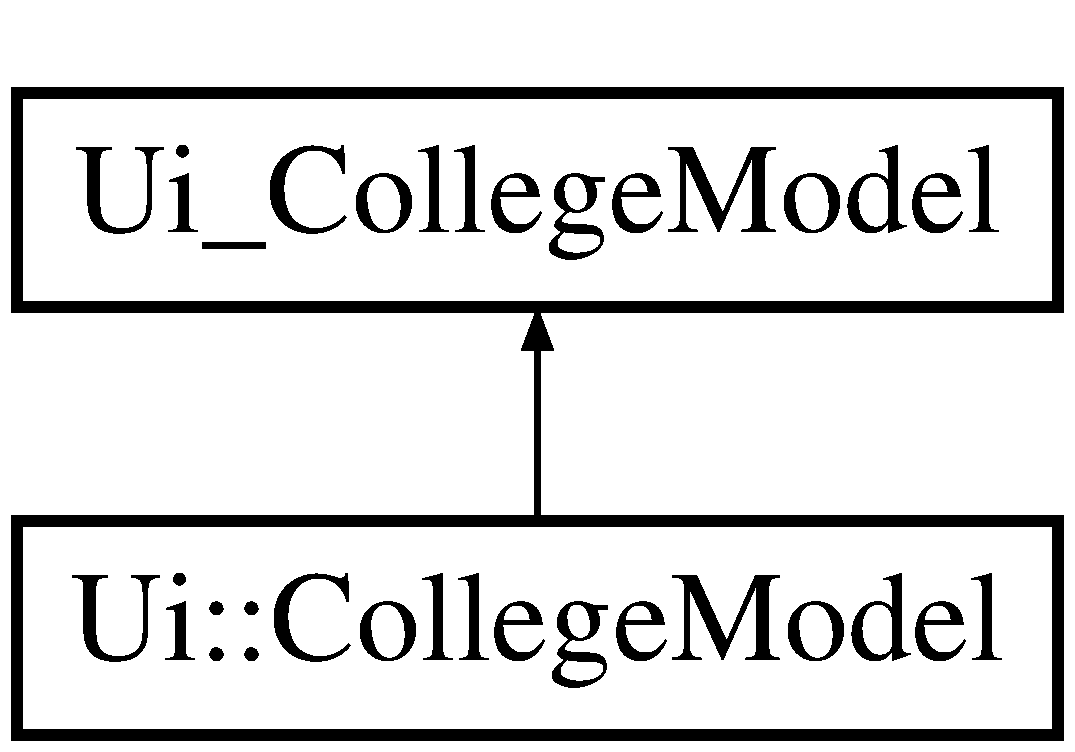
\includegraphics[height=2.000000cm]{class_ui_1_1_college_model}
\end{center}
\end{figure}
\subsection*{Additional Inherited Members}


The documentation for this class was generated from the following file\+:\begin{DoxyCompactItemize}
\item 
ui\+\_\+collegemodel.\+h\end{DoxyCompactItemize}

\hypertarget{class_college_model}{}\section{College\+Model Class Reference}
\label{class_college_model}\index{College\+Model@{College\+Model}}


The \mbox{\hyperlink{class_college_model}{College\+Model}} class The class that will process all the functionality of the UI and allow the user to properly plan their trip and make purchases.  




{\ttfamily \#include $<$collegemodel.\+h$>$}

Inheritance diagram for College\+Model\+:\begin{figure}[H]
\begin{center}
\leavevmode
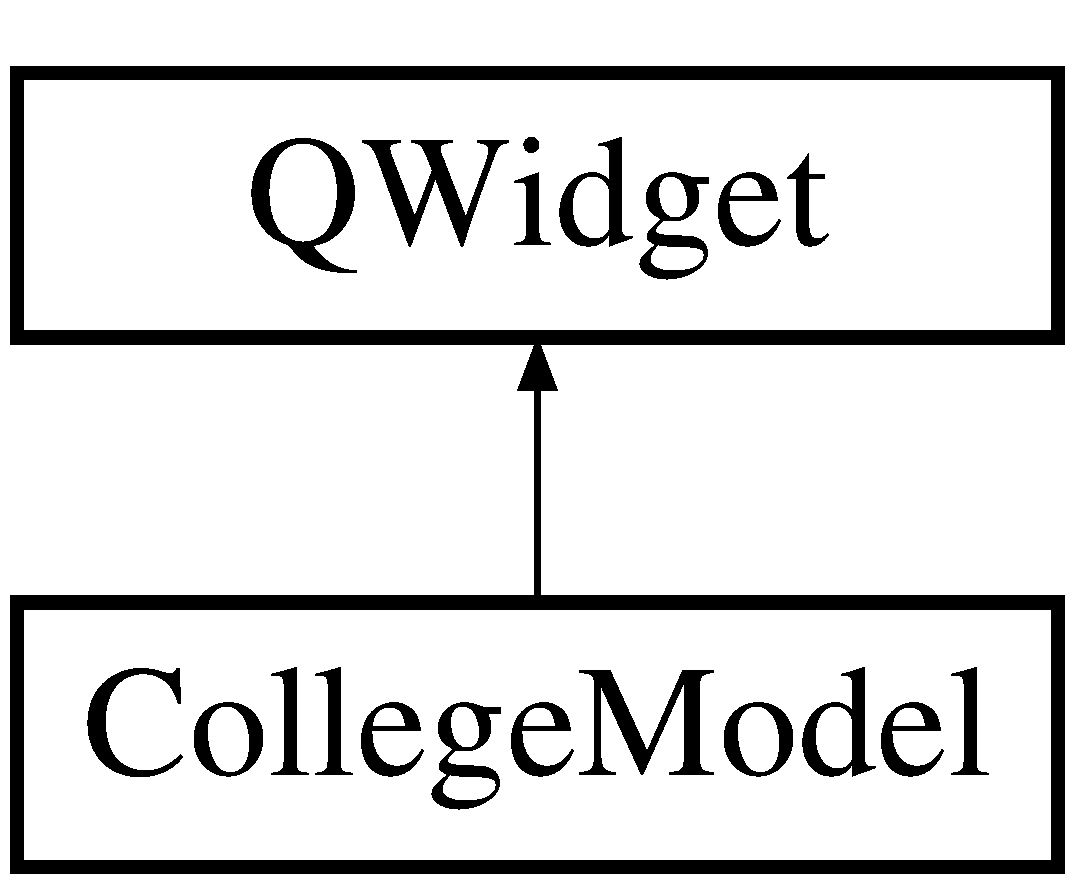
\includegraphics[height=2.000000cm]{class_college_model}
\end{center}
\end{figure}
\subsection*{Public Slots}
\begin{DoxyCompactItemize}
\item 
void \mbox{\hyperlink{class_college_model_a77fd4ae5151724440b68f236305ff74e}{souvenir\+Button\+Pressed}} ()
\begin{DoxyCompactList}\small\item\em Processes intermission between traversal. \end{DoxyCompactList}\end{DoxyCompactItemize}
\subsection*{Public Member Functions}
\begin{DoxyCompactItemize}
\item 
\mbox{\hyperlink{class_college_model_a028e4ea98b27a8d5fffafdb69a1d9e2d}{College\+Model}} (\mbox{\hyperlink{struct_college}{College}} college\+Clicked, bool asu\+Trip, Q\+Widget $\ast$parent=0)
\begin{DoxyCompactList}\small\item\em Constructor. \end{DoxyCompactList}\item 
\mbox{\hyperlink{class_college_model_a2edbda0635ecdd023e4d7ea8258f72e3}{$\sim$\+College\+Model}} ()
\begin{DoxyCompactList}\small\item\em Default Destructor. \end{DoxyCompactList}\item 
void \mbox{\hyperlink{class_college_model_a95322085a90304da8cbb265c80a3c3aa}{recursive\+Path\+Planner}} (\mbox{\hyperlink{struct_college}{College}} current\+College, Q\+Vector$<$ \mbox{\hyperlink{struct_college}{College}} $>$ \&most\+Efficient\+List)
\begin{DoxyCompactList}\small\item\em Recursive function to effectively plan the trip amongst colleges. \end{DoxyCompactList}\item 
void \mbox{\hyperlink{class_college_model_ab621eb530418fdcbd35a88911881504f}{get\+Trip\+Length}} ()
\begin{DoxyCompactList}\small\item\em Function to receive trip length from student. \end{DoxyCompactList}\item 
void \mbox{\hyperlink{class_college_model_aeabb600577c25bbe804849baa4875c14}{populate\+Souvenir\+Menu}} (int college\+ID)
\begin{DoxyCompactList}\small\item\em Populates menu with souvenir data to be purchased. \end{DoxyCompactList}\item 
void \mbox{\hyperlink{class_college_model_adad9674dbee23e82f64508cd1cfe2670}{clear\+Widgets}} (Q\+Layout $\ast$layout)
\begin{DoxyCompactList}\small\item\em Clears widgets to maintain integrity. \end{DoxyCompactList}\item 
bool \mbox{\hyperlink{class_college_model_a345c4e6868df90bed49e80b6783f5578}{vector\+Contains}} (Q\+Vector$<$ \mbox{\hyperlink{struct_college}{College}} $>$ colleges, \mbox{\hyperlink{struct_college}{College}} search\+Rest)
\begin{DoxyCompactList}\small\item\em Search function for college. \end{DoxyCompactList}\item 
void \mbox{\hyperlink{class_college_model_a0bf105af39d44c58b7acfc4600f739cf}{confirm\+Purchase}} (\mbox{\hyperlink{structsouvenir_item}{souvenir\+Item}} souvenir)
\begin{DoxyCompactList}\small\item\em Reassurance of purchase from student. \end{DoxyCompactList}\item 
void \mbox{\hyperlink{class_college_model_a6b2cca5127c7d95affe9870b1226a012}{update\+Cart}} (\mbox{\hyperlink{structsouvenir_item}{souvenir\+Item}} item)
\begin{DoxyCompactList}\small\item\em Adds item to cart and updates. \end{DoxyCompactList}\item 
void \mbox{\hyperlink{class_college_model_aec2e897e1a9e275308ed7889b7d94ef1}{delay}} (int n)
\begin{DoxyCompactList}\small\item\em \mbox{\hyperlink{class_college_model_aec2e897e1a9e275308ed7889b7d94ef1}{College\+Model\+::delay}} Helper timing function for loading page. \end{DoxyCompactList}\end{DoxyCompactItemize}
\subsection*{Protected Slots}
\begin{DoxyCompactItemize}
\item 
void \mbox{\hyperlink{class_college_model_ac37d99bb60d755ef0539d8e6c4481ab7}{loading\+Page}} ()
\begin{DoxyCompactList}\small\item\em Timing function. \end{DoxyCompactList}\end{DoxyCompactItemize}


\subsection{Detailed Description}
The \mbox{\hyperlink{class_college_model}{College\+Model}} class The class that will process all the functionality of the UI and allow the user to properly plan their trip and make purchases. 

\subsection{Constructor \& Destructor Documentation}
\mbox{\Hypertarget{class_college_model_a028e4ea98b27a8d5fffafdb69a1d9e2d}\label{class_college_model_a028e4ea98b27a8d5fffafdb69a1d9e2d}} 
\index{College\+Model@{College\+Model}!College\+Model@{College\+Model}}
\index{College\+Model@{College\+Model}!College\+Model@{College\+Model}}
\subsubsection{\texorpdfstring{College\+Model()}{CollegeModel()}}
{\footnotesize\ttfamily College\+Model\+::\+College\+Model (\begin{DoxyParamCaption}\item[{\mbox{\hyperlink{struct_college}{College}}}]{college\+Clicked,  }\item[{bool}]{asu\+Trip,  }\item[{Q\+Widget $\ast$}]{parent = {\ttfamily 0} }\end{DoxyParamCaption})\hspace{0.3cm}{\ttfamily [explicit]}}



Constructor. 

\mbox{\hyperlink{class_college_model_a028e4ea98b27a8d5fffafdb69a1d9e2d}{College\+Model\+::\+College\+Model}}.

The \mbox{\hyperlink{struct_college}{College}} User-\/\+Interface 
\begin{DoxyParams}{Parameters}
{\em college\+Clicked} & -\/ A struct argument \\
\hline
{\em asu\+Trip} & -\/ bool for starting point \\
\hline
{\em parent} & \\
\hline
\end{DoxyParams}
\mbox{\Hypertarget{class_college_model_a2edbda0635ecdd023e4d7ea8258f72e3}\label{class_college_model_a2edbda0635ecdd023e4d7ea8258f72e3}} 
\index{College\+Model@{College\+Model}!````~College\+Model@{$\sim$\+College\+Model}}
\index{````~College\+Model@{$\sim$\+College\+Model}!College\+Model@{College\+Model}}
\subsubsection{\texorpdfstring{$\sim$\+College\+Model()}{~CollegeModel()}}
{\footnotesize\ttfamily College\+Model\+::$\sim$\+College\+Model (\begin{DoxyParamCaption}{ }\end{DoxyParamCaption})}



Default Destructor. 

\mbox{\hyperlink{class_college_model_a2edbda0635ecdd023e4d7ea8258f72e3}{College\+Model\+::$\sim$\+College\+Model}}.

Default Constructor 

\subsection{Member Function Documentation}
\mbox{\Hypertarget{class_college_model_adad9674dbee23e82f64508cd1cfe2670}\label{class_college_model_adad9674dbee23e82f64508cd1cfe2670}} 
\index{College\+Model@{College\+Model}!clear\+Widgets@{clear\+Widgets}}
\index{clear\+Widgets@{clear\+Widgets}!College\+Model@{College\+Model}}
\subsubsection{\texorpdfstring{clear\+Widgets()}{clearWidgets()}}
{\footnotesize\ttfamily void College\+Model\+::clear\+Widgets (\begin{DoxyParamCaption}\item[{Q\+Layout $\ast$}]{layout }\end{DoxyParamCaption})}



Clears widgets to maintain integrity. 

\mbox{\hyperlink{class_college_model_adad9674dbee23e82f64508cd1cfe2670}{College\+Model\+::clear\+Widgets}}.


\begin{DoxyParams}{Parameters}
{\em layout} & -\/ Widget to be cleared argument \\
\hline
\end{DoxyParams}
\mbox{\Hypertarget{class_college_model_a0bf105af39d44c58b7acfc4600f739cf}\label{class_college_model_a0bf105af39d44c58b7acfc4600f739cf}} 
\index{College\+Model@{College\+Model}!confirm\+Purchase@{confirm\+Purchase}}
\index{confirm\+Purchase@{confirm\+Purchase}!College\+Model@{College\+Model}}
\subsubsection{\texorpdfstring{confirm\+Purchase()}{confirmPurchase()}}
{\footnotesize\ttfamily void College\+Model\+::confirm\+Purchase (\begin{DoxyParamCaption}\item[{\mbox{\hyperlink{structsouvenir_item}{souvenir\+Item}}}]{souvenir }\end{DoxyParamCaption})}



Reassurance of purchase from student. 

\mbox{\hyperlink{class_college_model_a0bf105af39d44c58b7acfc4600f739cf}{College\+Model\+::confirm\+Purchase}} Confirms if the user wants to purchase the item they have selected for reassurance.


\begin{DoxyParams}{Parameters}
{\em souvenir} & -\/ A struct argument \\
\hline
\end{DoxyParams}
\mbox{\Hypertarget{class_college_model_aec2e897e1a9e275308ed7889b7d94ef1}\label{class_college_model_aec2e897e1a9e275308ed7889b7d94ef1}} 
\index{College\+Model@{College\+Model}!delay@{delay}}
\index{delay@{delay}!College\+Model@{College\+Model}}
\subsubsection{\texorpdfstring{delay()}{delay()}}
{\footnotesize\ttfamily void College\+Model\+::delay (\begin{DoxyParamCaption}\item[{int}]{n }\end{DoxyParamCaption})}



\mbox{\hyperlink{class_college_model_aec2e897e1a9e275308ed7889b7d94ef1}{College\+Model\+::delay}} Helper timing function for loading page. 


\begin{DoxyParams}{Parameters}
{\em n} & -\/ Amount of seconds to delay \\
\hline
\end{DoxyParams}
\mbox{\Hypertarget{class_college_model_ab621eb530418fdcbd35a88911881504f}\label{class_college_model_ab621eb530418fdcbd35a88911881504f}} 
\index{College\+Model@{College\+Model}!get\+Trip\+Length@{get\+Trip\+Length}}
\index{get\+Trip\+Length@{get\+Trip\+Length}!College\+Model@{College\+Model}}
\subsubsection{\texorpdfstring{get\+Trip\+Length()}{getTripLength()}}
{\footnotesize\ttfamily void College\+Model\+::get\+Trip\+Length (\begin{DoxyParamCaption}{ }\end{DoxyParamCaption})}



Function to receive trip length from student. 

\mbox{\hyperlink{class_college_model_ab621eb530418fdcbd35a88911881504f}{College\+Model\+::get\+Trip\+Length}} prompts user for trip length based on total colleges in database. \mbox{\Hypertarget{class_college_model_ac37d99bb60d755ef0539d8e6c4481ab7}\label{class_college_model_ac37d99bb60d755ef0539d8e6c4481ab7}} 
\index{College\+Model@{College\+Model}!loading\+Page@{loading\+Page}}
\index{loading\+Page@{loading\+Page}!College\+Model@{College\+Model}}
\subsubsection{\texorpdfstring{loading\+Page}{loadingPage}}
{\footnotesize\ttfamily void College\+Model\+::loading\+Page (\begin{DoxyParamCaption}{ }\end{DoxyParamCaption})\hspace{0.3cm}{\ttfamily [protected]}, {\ttfamily [slot]}}



Timing function. 

\mbox{\hyperlink{class_college_model_ac37d99bb60d755ef0539d8e6c4481ab7}{College\+Model\+::loading\+Page}} Brief intermission when traveling. \mbox{\Hypertarget{class_college_model_aeabb600577c25bbe804849baa4875c14}\label{class_college_model_aeabb600577c25bbe804849baa4875c14}} 
\index{College\+Model@{College\+Model}!populate\+Souvenir\+Menu@{populate\+Souvenir\+Menu}}
\index{populate\+Souvenir\+Menu@{populate\+Souvenir\+Menu}!College\+Model@{College\+Model}}
\subsubsection{\texorpdfstring{populate\+Souvenir\+Menu()}{populateSouvenirMenu()}}
{\footnotesize\ttfamily void College\+Model\+::populate\+Souvenir\+Menu (\begin{DoxyParamCaption}\item[{int}]{college\+ID }\end{DoxyParamCaption})}



Populates menu with souvenir data to be purchased. 

\mbox{\hyperlink{class_college_model_aeabb600577c25bbe804849baa4875c14}{College\+Model\+::populate\+Souvenir\+Menu}} populates layout with souvenir buttons representing the databases souvenir items for current college that the student can interact with to add souvenirs to their cart.


\begin{DoxyParams}{Parameters}
{\em college\+ID} & -\/ A struct argument \\
\hline
\end{DoxyParams}
\mbox{\Hypertarget{class_college_model_a95322085a90304da8cbb265c80a3c3aa}\label{class_college_model_a95322085a90304da8cbb265c80a3c3aa}} 
\index{College\+Model@{College\+Model}!recursive\+Path\+Planner@{recursive\+Path\+Planner}}
\index{recursive\+Path\+Planner@{recursive\+Path\+Planner}!College\+Model@{College\+Model}}
\subsubsection{\texorpdfstring{recursive\+Path\+Planner()}{recursivePathPlanner()}}
{\footnotesize\ttfamily void College\+Model\+::recursive\+Path\+Planner (\begin{DoxyParamCaption}\item[{\mbox{\hyperlink{struct_college}{College}}}]{current\+College,  }\item[{Q\+Vector$<$ \mbox{\hyperlink{struct_college}{College}} $>$ \&}]{most\+Efficient\+List }\end{DoxyParamCaption})}



Recursive function to effectively plan the trip amongst colleges. 

\mbox{\hyperlink{class_college_model_a95322085a90304da8cbb265c80a3c3aa}{College\+Model\+::recursive\+Path\+Planner}} Recursively travels from each college to the next based upon the shortest distance between each of the colleges, thens stores the traversal order into a Q\+Vector of colleges to be used for the student\textquotesingle{}s trip.


\begin{DoxyParams}{Parameters}
{\em current\+College} & -\/ A struct argument \\
\hline
{\em most\+Efficient\+List} & -\/ A Q\+Vector of structs \\
\hline
\end{DoxyParams}
\mbox{\Hypertarget{class_college_model_a77fd4ae5151724440b68f236305ff74e}\label{class_college_model_a77fd4ae5151724440b68f236305ff74e}} 
\index{College\+Model@{College\+Model}!souvenir\+Button\+Pressed@{souvenir\+Button\+Pressed}}
\index{souvenir\+Button\+Pressed@{souvenir\+Button\+Pressed}!College\+Model@{College\+Model}}
\subsubsection{\texorpdfstring{souvenir\+Button\+Pressed}{souvenirButtonPressed}}
{\footnotesize\ttfamily void College\+Model\+::souvenir\+Button\+Pressed (\begin{DoxyParamCaption}{ }\end{DoxyParamCaption})\hspace{0.3cm}{\ttfamily [slot]}}



Processes intermission between traversal. 

\mbox{\hyperlink{class_college_model_a77fd4ae5151724440b68f236305ff74e}{College\+Model\+::souvenir\+Button\+Pressed}} Function to use data from the souvenir buttons to add item from database into their transactions. \mbox{\Hypertarget{class_college_model_a6b2cca5127c7d95affe9870b1226a012}\label{class_college_model_a6b2cca5127c7d95affe9870b1226a012}} 
\index{College\+Model@{College\+Model}!update\+Cart@{update\+Cart}}
\index{update\+Cart@{update\+Cart}!College\+Model@{College\+Model}}
\subsubsection{\texorpdfstring{update\+Cart()}{updateCart()}}
{\footnotesize\ttfamily void College\+Model\+::update\+Cart (\begin{DoxyParamCaption}\item[{\mbox{\hyperlink{structsouvenir_item}{souvenir\+Item}}}]{item }\end{DoxyParamCaption})}



Adds item to cart and updates. 

\mbox{\hyperlink{class_college_model_a6b2cca5127c7d95affe9870b1226a012}{College\+Model\+::update\+Cart}} Updates student\textquotesingle{}s cart to ensure it is accurate and all items are proper.


\begin{DoxyParams}{Parameters}
{\em item} & -\/ A struct argument \\
\hline
\end{DoxyParams}
\mbox{\Hypertarget{class_college_model_a345c4e6868df90bed49e80b6783f5578}\label{class_college_model_a345c4e6868df90bed49e80b6783f5578}} 
\index{College\+Model@{College\+Model}!vector\+Contains@{vector\+Contains}}
\index{vector\+Contains@{vector\+Contains}!College\+Model@{College\+Model}}
\subsubsection{\texorpdfstring{vector\+Contains()}{vectorContains()}}
{\footnotesize\ttfamily bool College\+Model\+::vector\+Contains (\begin{DoxyParamCaption}\item[{Q\+Vector$<$ \mbox{\hyperlink{struct_college}{College}} $>$}]{colleges,  }\item[{\mbox{\hyperlink{struct_college}{College}}}]{search\+Rest }\end{DoxyParamCaption})}



Search function for college. 

\mbox{\hyperlink{class_college_model_a345c4e6868df90bed49e80b6783f5578}{College\+Model\+::vector\+Contains}} Scans vector of colleges if a specified college argument is present.


\begin{DoxyParams}{Parameters}
{\em colleges} & -\/ A Q\+Vector of structs \\
\hline
{\em search\+Rest} & -\/ A struct argument \\
\hline
\end{DoxyParams}
\begin{DoxyReturn}{Returns}
bool of if searched college was found 
\end{DoxyReturn}


The documentation for this class was generated from the following files\+:\begin{DoxyCompactItemize}
\item 
collegemodel.\+h\item 
collegemodel.\+cpp\end{DoxyCompactItemize}

\hypertarget{classdb_manager}{}\section{db\+Manager Class Reference}
\label{classdb_manager}\index{db\+Manager@{db\+Manager}}


The \mbox{\hyperlink{classdb_manager}{db\+Manager}} class Class to handle all functionality of a S\+Q\+Lite database. Allows only a single instance to be created and uses that instance throughout execution. All data will be represented in Q\+Vectors and queries.  




{\ttfamily \#include $<$dbmanager.\+h$>$}

\subsection*{Public Member Functions}
\begin{DoxyCompactItemize}
\item 
\mbox{\Hypertarget{classdb_manager_a6980cc0fa5fdc50934944c6f17b6980a}\label{classdb_manager_a6980cc0fa5fdc50934944c6f17b6980a}} 
void \mbox{\hyperlink{classdb_manager_a6980cc0fa5fdc50934944c6f17b6980a}{initialize\+DB}} ()
\begin{DoxyCompactList}\small\item\em \mbox{\hyperlink{classdb_manager_a6980cc0fa5fdc50934944c6f17b6980a}{db\+Manager\+::initialize\+DB}} Initializes data if not present \end{DoxyCompactList}\item 
void \mbox{\hyperlink{classdb_manager_a4170bc104b663300dee1fd7390a6ae63}{close\+Database}} ()
\begin{DoxyCompactList}\small\item\em Initializes instance of database. \end{DoxyCompactList}\item 
int \mbox{\hyperlink{classdb_manager_ae211811d8431bd57bd250c2ab753f691}{get\+Total\+Colleges}} ()
\begin{DoxyCompactList}\small\item\em Receives pointer to database for access. \end{DoxyCompactList}\item 
Q\+Vector$<$ \mbox{\hyperlink{struct_college}{College}} $>$ \mbox{\hyperlink{classdb_manager_aad9d2f24ac9c74728393502b6c04a0b8}{get\+Colleges}} ()
\begin{DoxyCompactList}\small\item\em Receives number of colleges in database. \end{DoxyCompactList}\item 
Q\+Vector$<$ \mbox{\hyperlink{structsouvenir_item}{souvenir\+Item}} $>$ \mbox{\hyperlink{classdb_manager_a91281dfbeb41cebfa8a633e3a7e12a5e}{get\+Souvenirs\+By\+College\+ID}} (int college\+ID)
\begin{DoxyCompactList}\small\item\em Function to get every college in database. \end{DoxyCompactList}\item 
\mbox{\hyperlink{struct_college}{College}} \mbox{\hyperlink{classdb_manager_a1ad8ef74ddb1a0022a1598ef9e60cd6f}{get\+College\+By\+ID}} (int college\+\_\+\+ID)
\begin{DoxyCompactList}\small\item\em Searches database for souvenir by college ID. \end{DoxyCompactList}\item 
\mbox{\hyperlink{structsouvenir_item}{souvenir\+Item}} \mbox{\hyperlink{classdb_manager_a005ba0700501bd4c601a79248607f2b6}{get\+Souvenir\+By\+ID}} (int souvenir\+Item\+\_\+\+ID)
\begin{DoxyCompactList}\small\item\em Searches for college by college ID. \end{DoxyCompactList}\item 
Q\+Vector$<$ \mbox{\hyperlink{struct_distance}{Distance}} $>$ \mbox{\hyperlink{classdb_manager_aaa56ad9c1a84cd0063efa1551b297138}{get\+Distances\+From}} (int source\+College\+\_\+\+ID)
\begin{DoxyCompactList}\small\item\em Searches for souvenir by college ID. \end{DoxyCompactList}\item 
bool \mbox{\hyperlink{classdb_manager_a0ce2c2fa322e30e512165509811544fa}{authenticate\+Admin\+Login\+Request}} (Q\+String name, Q\+String password)
\begin{DoxyCompactList}\small\item\em Checks distances between colleges. \end{DoxyCompactList}\item 
void \mbox{\hyperlink{classdb_manager_ae466201599ce67617d769a1196714bf1}{add\+College}} (\mbox{\hyperlink{struct_college}{College}} college, Q\+Vector$<$ \mbox{\hyperlink{struct_distance}{Distance}} $>$ distances)
\begin{DoxyCompactList}\small\item\em Validates credentials to database credentials. \end{DoxyCompactList}\item 
void \mbox{\hyperlink{classdb_manager_aa52b30e936de3c8c7b561c6d6c6a4cd6}{add\+Souvenir\+Item}} (\mbox{\hyperlink{structsouvenir_item}{souvenir\+Item}} new\+Souvenir, \mbox{\hyperlink{struct_college}{College}} to\+Add\+To)
\begin{DoxyCompactList}\small\item\em Adds college to database. \end{DoxyCompactList}\item 
void \mbox{\hyperlink{classdb_manager_a4d1f437fbf2bed7786324a8dcf639a4a}{modify\+Souvenir\+Item}} (\mbox{\hyperlink{structsouvenir_item}{souvenir\+Item}} new\+Souvenir)
\begin{DoxyCompactList}\small\item\em Adds souvenir item to database. \end{DoxyCompactList}\item 
void \mbox{\hyperlink{classdb_manager_a97da73c78035103e648836dbfb927786}{delete\+Souvenir\+Item}} (\mbox{\hyperlink{structsouvenir_item}{souvenir\+Item}} deleted\+Item)
\begin{DoxyCompactList}\small\item\em Modifies information of specific souvenir item in database. \end{DoxyCompactList}\end{DoxyCompactItemize}
\subsection*{Static Public Member Functions}
\begin{DoxyCompactItemize}
\item 
static \mbox{\hyperlink{classdb_manager}{db\+Manager}} $\ast$ \mbox{\hyperlink{classdb_manager_a0b96aeab4f66563db74711be1dfc1edb}{get\+Instance}} ()
\begin{DoxyCompactList}\small\item\em Closes connection upon termination. \end{DoxyCompactList}\end{DoxyCompactItemize}


\subsection{Detailed Description}
The \mbox{\hyperlink{classdb_manager}{db\+Manager}} class Class to handle all functionality of a S\+Q\+Lite database. Allows only a single instance to be created and uses that instance throughout execution. All data will be represented in Q\+Vectors and queries. 

The Database Manager 

\subsection{Member Function Documentation}
\mbox{\Hypertarget{classdb_manager_ae466201599ce67617d769a1196714bf1}\label{classdb_manager_ae466201599ce67617d769a1196714bf1}} 
\index{db\+Manager@{db\+Manager}!add\+College@{add\+College}}
\index{add\+College@{add\+College}!db\+Manager@{db\+Manager}}
\subsubsection{\texorpdfstring{add\+College()}{addCollege()}}
{\footnotesize\ttfamily void db\+Manager\+::add\+College (\begin{DoxyParamCaption}\item[{\mbox{\hyperlink{struct_college}{College}}}]{college,  }\item[{Q\+Vector$<$ \mbox{\hyperlink{struct_distance}{Distance}} $>$}]{distances }\end{DoxyParamCaption})}



Validates credentials to database credentials. 

\mbox{\hyperlink{classdb_manager_ae466201599ce67617d769a1196714bf1}{db\+Manager\+::add\+College}} Will use input college information to add it to databse

To add a new college to database 
\begin{DoxyParams}{Parameters}
{\em college} & -\/ A struct argument \\
\hline
{\em distances} & -\/ A Q\+Vector argument \\
\hline
\end{DoxyParams}
\mbox{\Hypertarget{classdb_manager_aa52b30e936de3c8c7b561c6d6c6a4cd6}\label{classdb_manager_aa52b30e936de3c8c7b561c6d6c6a4cd6}} 
\index{db\+Manager@{db\+Manager}!add\+Souvenir\+Item@{add\+Souvenir\+Item}}
\index{add\+Souvenir\+Item@{add\+Souvenir\+Item}!db\+Manager@{db\+Manager}}
\subsubsection{\texorpdfstring{add\+Souvenir\+Item()}{addSouvenirItem()}}
{\footnotesize\ttfamily void db\+Manager\+::add\+Souvenir\+Item (\begin{DoxyParamCaption}\item[{\mbox{\hyperlink{structsouvenir_item}{souvenir\+Item}}}]{new\+Souvenir,  }\item[{\mbox{\hyperlink{struct_college}{College}}}]{to\+Add\+To }\end{DoxyParamCaption})}



Adds college to database. 

\mbox{\hyperlink{classdb_manager_aa52b30e936de3c8c7b561c6d6c6a4cd6}{db\+Manager\+::add\+Souvenir\+Item}} Adds souvenir item to records based on input information

To add souvenir item to database 
\begin{DoxyParams}{Parameters}
{\em new\+Souvenir} & -\/ A struct argument \\
\hline
{\em to\+Add\+To} & -\/ A struct argument \\
\hline
\end{DoxyParams}
\mbox{\Hypertarget{classdb_manager_a0ce2c2fa322e30e512165509811544fa}\label{classdb_manager_a0ce2c2fa322e30e512165509811544fa}} 
\index{db\+Manager@{db\+Manager}!authenticate\+Admin\+Login\+Request@{authenticate\+Admin\+Login\+Request}}
\index{authenticate\+Admin\+Login\+Request@{authenticate\+Admin\+Login\+Request}!db\+Manager@{db\+Manager}}
\subsubsection{\texorpdfstring{authenticate\+Admin\+Login\+Request()}{authenticateAdminLoginRequest()}}
{\footnotesize\ttfamily bool db\+Manager\+::authenticate\+Admin\+Login\+Request (\begin{DoxyParamCaption}\item[{Q\+String}]{name,  }\item[{Q\+String}]{password }\end{DoxyParamCaption})}



Checks distances between colleges. 

A function to verify login request of admin.

authenticate\+Admin\+Login\+Request Will take the username and password entered and compare it to the key stored to verify access. 
\begin{DoxyParams}{Parameters}
{\em username} & -\/ A Q\+String argument \\
\hline
{\em passsword} & -\/ A Q\+String argument \\
\hline
\end{DoxyParams}
\begin{DoxyReturn}{Returns}
A boolean that is true if the entered information is identical 
\end{DoxyReturn}
\mbox{\Hypertarget{classdb_manager_a4170bc104b663300dee1fd7390a6ae63}\label{classdb_manager_a4170bc104b663300dee1fd7390a6ae63}} 
\index{db\+Manager@{db\+Manager}!close\+Database@{close\+Database}}
\index{close\+Database@{close\+Database}!db\+Manager@{db\+Manager}}
\subsubsection{\texorpdfstring{close\+Database()}{closeDatabase()}}
{\footnotesize\ttfamily void db\+Manager\+::close\+Database (\begin{DoxyParamCaption}{ }\end{DoxyParamCaption})}



Initializes instance of database. 

\mbox{\hyperlink{classdb_manager_a4170bc104b663300dee1fd7390a6ae63}{db\+Manager\+::close\+Database}} removes connection to database

Closes connection \mbox{\Hypertarget{classdb_manager_a97da73c78035103e648836dbfb927786}\label{classdb_manager_a97da73c78035103e648836dbfb927786}} 
\index{db\+Manager@{db\+Manager}!delete\+Souvenir\+Item@{delete\+Souvenir\+Item}}
\index{delete\+Souvenir\+Item@{delete\+Souvenir\+Item}!db\+Manager@{db\+Manager}}
\subsubsection{\texorpdfstring{delete\+Souvenir\+Item()}{deleteSouvenirItem()}}
{\footnotesize\ttfamily void db\+Manager\+::delete\+Souvenir\+Item (\begin{DoxyParamCaption}\item[{\mbox{\hyperlink{structsouvenir_item}{souvenir\+Item}}}]{deleted\+Item }\end{DoxyParamCaption})}



Modifies information of specific souvenir item in database. 

\mbox{\hyperlink{classdb_manager_a97da73c78035103e648836dbfb927786}{db\+Manager\+::delete\+Souvenir\+Item}} Will take item and delete it from database records

Deletes souvenir from database 
\begin{DoxyParams}{Parameters}
{\em deleted\+Item} & \\
\hline
\end{DoxyParams}
\mbox{\Hypertarget{classdb_manager_a1ad8ef74ddb1a0022a1598ef9e60cd6f}\label{classdb_manager_a1ad8ef74ddb1a0022a1598ef9e60cd6f}} 
\index{db\+Manager@{db\+Manager}!get\+College\+By\+ID@{get\+College\+By\+ID}}
\index{get\+College\+By\+ID@{get\+College\+By\+ID}!db\+Manager@{db\+Manager}}
\subsubsection{\texorpdfstring{get\+College\+By\+I\+D()}{getCollegeByID()}}
{\footnotesize\ttfamily \mbox{\hyperlink{struct_college}{College}} db\+Manager\+::get\+College\+By\+ID (\begin{DoxyParamCaption}\item[{int}]{college\+\_\+\+ID }\end{DoxyParamCaption})}



Searches database for souvenir by college ID. 

\mbox{\hyperlink{classdb_manager_a1ad8ef74ddb1a0022a1598ef9e60cd6f}{db\+Manager\+::get\+College\+By\+ID}}

To find college by associated ID 
\begin{DoxyParams}{Parameters}
{\em college\+\_\+\+ID} & -\/ An integer argument \\
\hline
\end{DoxyParams}
\begin{DoxyReturn}{Returns}

\end{DoxyReturn}
\mbox{\Hypertarget{classdb_manager_aad9d2f24ac9c74728393502b6c04a0b8}\label{classdb_manager_aad9d2f24ac9c74728393502b6c04a0b8}} 
\index{db\+Manager@{db\+Manager}!get\+Colleges@{get\+Colleges}}
\index{get\+Colleges@{get\+Colleges}!db\+Manager@{db\+Manager}}
\subsubsection{\texorpdfstring{get\+Colleges()}{getColleges()}}
{\footnotesize\ttfamily Q\+Vector$<$ \mbox{\hyperlink{struct_college}{College}} $>$ db\+Manager\+::get\+Colleges (\begin{DoxyParamCaption}{ }\end{DoxyParamCaption})}



Receives number of colleges in database. 

\mbox{\hyperlink{classdb_manager_aad9d2f24ac9c74728393502b6c04a0b8}{db\+Manager\+::get\+Colleges}}

Function to get all colleges in database \begin{DoxyReturn}{Returns}
Q\+Vector of colleges 
\end{DoxyReturn}
\mbox{\Hypertarget{classdb_manager_aaa56ad9c1a84cd0063efa1551b297138}\label{classdb_manager_aaa56ad9c1a84cd0063efa1551b297138}} 
\index{db\+Manager@{db\+Manager}!get\+Distances\+From@{get\+Distances\+From}}
\index{get\+Distances\+From@{get\+Distances\+From}!db\+Manager@{db\+Manager}}
\subsubsection{\texorpdfstring{get\+Distances\+From()}{getDistancesFrom()}}
{\footnotesize\ttfamily Q\+Vector$<$ \mbox{\hyperlink{struct_distance}{Distance}} $>$ db\+Manager\+::get\+Distances\+From (\begin{DoxyParamCaption}\item[{int}]{source\+College\+\_\+\+ID }\end{DoxyParamCaption})}



Searches for souvenir by college ID. 

To get the colleges to other colleges.

get\+Distances\+From Will take in the colleges ID and match it with is corresponding distances list and return it for use. 
\begin{DoxyParams}{Parameters}
{\em source\+College\+\_\+\+ID} & -\/ An integer argument \\
\hline
\end{DoxyParams}
\begin{DoxyReturn}{Returns}
A Q\+Vector of the distances of that college 
\end{DoxyReturn}
\mbox{\Hypertarget{classdb_manager_a0b96aeab4f66563db74711be1dfc1edb}\label{classdb_manager_a0b96aeab4f66563db74711be1dfc1edb}} 
\index{db\+Manager@{db\+Manager}!get\+Instance@{get\+Instance}}
\index{get\+Instance@{get\+Instance}!db\+Manager@{db\+Manager}}
\subsubsection{\texorpdfstring{get\+Instance()}{getInstance()}}
{\footnotesize\ttfamily \mbox{\hyperlink{classdb_manager}{db\+Manager}} $\ast$ db\+Manager\+::get\+Instance (\begin{DoxyParamCaption}{ }\end{DoxyParamCaption})\hspace{0.3cm}{\ttfamily [static]}}



Closes connection upon termination. 

\mbox{\hyperlink{classdb_manager_a0b96aeab4f66563db74711be1dfc1edb}{db\+Manager\+::get\+Instance}} Used for everytime database access is needed

To access database \begin{DoxyReturn}{Returns}
pointer to database 
\end{DoxyReturn}
\mbox{\Hypertarget{classdb_manager_a005ba0700501bd4c601a79248607f2b6}\label{classdb_manager_a005ba0700501bd4c601a79248607f2b6}} 
\index{db\+Manager@{db\+Manager}!get\+Souvenir\+By\+ID@{get\+Souvenir\+By\+ID}}
\index{get\+Souvenir\+By\+ID@{get\+Souvenir\+By\+ID}!db\+Manager@{db\+Manager}}
\subsubsection{\texorpdfstring{get\+Souvenir\+By\+I\+D()}{getSouvenirByID()}}
{\footnotesize\ttfamily \mbox{\hyperlink{structsouvenir_item}{souvenir\+Item}} db\+Manager\+::get\+Souvenir\+By\+ID (\begin{DoxyParamCaption}\item[{int}]{souvenir\+Item\+\_\+\+ID }\end{DoxyParamCaption})}



Searches for college by college ID. 

\mbox{\hyperlink{classdb_manager_a005ba0700501bd4c601a79248607f2b6}{db\+Manager\+::get\+Souvenir\+By\+ID}} Searches database by specific souvenir ID

To find souvenir by ID 
\begin{DoxyParams}{Parameters}
{\em souvenir\+Item\+\_\+\+ID} & -\/ An integer argument \\
\hline
\end{DoxyParams}
\begin{DoxyReturn}{Returns}

\end{DoxyReturn}
\mbox{\Hypertarget{classdb_manager_a91281dfbeb41cebfa8a633e3a7e12a5e}\label{classdb_manager_a91281dfbeb41cebfa8a633e3a7e12a5e}} 
\index{db\+Manager@{db\+Manager}!get\+Souvenirs\+By\+College\+ID@{get\+Souvenirs\+By\+College\+ID}}
\index{get\+Souvenirs\+By\+College\+ID@{get\+Souvenirs\+By\+College\+ID}!db\+Manager@{db\+Manager}}
\subsubsection{\texorpdfstring{get\+Souvenirs\+By\+College\+I\+D()}{getSouvenirsByCollegeID()}}
{\footnotesize\ttfamily Q\+Vector$<$ \mbox{\hyperlink{structsouvenir_item}{souvenir\+Item}} $>$ db\+Manager\+::get\+Souvenirs\+By\+College\+ID (\begin{DoxyParamCaption}\item[{int}]{college\+ID }\end{DoxyParamCaption})}



Function to get every college in database. 

\mbox{\hyperlink{classdb_manager_a91281dfbeb41cebfa8a633e3a7e12a5e}{db\+Manager\+::get\+Souvenirs\+By\+College\+ID}}

To find souvenirs of a college 
\begin{DoxyParams}{Parameters}
{\em college\+ID} & -\/ An integer argument \\
\hline
\end{DoxyParams}
\begin{DoxyReturn}{Returns}
Q\+Vector of souvenirs that college has associated with it 
\end{DoxyReturn}
\mbox{\Hypertarget{classdb_manager_ae211811d8431bd57bd250c2ab753f691}\label{classdb_manager_ae211811d8431bd57bd250c2ab753f691}} 
\index{db\+Manager@{db\+Manager}!get\+Total\+Colleges@{get\+Total\+Colleges}}
\index{get\+Total\+Colleges@{get\+Total\+Colleges}!db\+Manager@{db\+Manager}}
\subsubsection{\texorpdfstring{get\+Total\+Colleges()}{getTotalColleges()}}
{\footnotesize\ttfamily int db\+Manager\+::get\+Total\+Colleges (\begin{DoxyParamCaption}{ }\end{DoxyParamCaption})}



Receives pointer to database for access. 

\mbox{\hyperlink{classdb_manager_ae211811d8431bd57bd250c2ab753f691}{db\+Manager\+::get\+Total\+Colleges}}

\begin{DoxyReturn}{Returns}
size of college records 
\end{DoxyReturn}
\mbox{\Hypertarget{classdb_manager_a4d1f437fbf2bed7786324a8dcf639a4a}\label{classdb_manager_a4d1f437fbf2bed7786324a8dcf639a4a}} 
\index{db\+Manager@{db\+Manager}!modify\+Souvenir\+Item@{modify\+Souvenir\+Item}}
\index{modify\+Souvenir\+Item@{modify\+Souvenir\+Item}!db\+Manager@{db\+Manager}}
\subsubsection{\texorpdfstring{modify\+Souvenir\+Item()}{modifySouvenirItem()}}
{\footnotesize\ttfamily void db\+Manager\+::modify\+Souvenir\+Item (\begin{DoxyParamCaption}\item[{\mbox{\hyperlink{structsouvenir_item}{souvenir\+Item}}}]{new\+Souvenir\+Item }\end{DoxyParamCaption})}



Adds souvenir item to database. 

\mbox{\hyperlink{classdb_manager_a4d1f437fbf2bed7786324a8dcf639a4a}{db\+Manager\+::modify\+Souvenir\+Item}} Changes record data fro given souvenir item

To modify souvenir information 
\begin{DoxyParams}{Parameters}
{\em new\+Souvenir\+Item} & -\/ A struct argument \\
\hline
\end{DoxyParams}


The documentation for this class was generated from the following files\+:\begin{DoxyCompactItemize}
\item 
dbmanager.\+h\item 
dbmanager.\+cpp\end{DoxyCompactItemize}

\hypertarget{struct_distance}{}\section{Distance Struct Reference}
\label{struct_distance}\index{Distance@{Distance}}


The \mbox{\hyperlink{struct_distance}{Distance}} struct Stores distances between two colleges.  




{\ttfamily \#include $<$mainwindow.\+h$>$}

\subsection*{Public Attributes}
\begin{DoxyCompactItemize}
\item 
\mbox{\Hypertarget{struct_distance_a11eea19a1d9b2dc334ea53101994a6f0}\label{struct_distance_a11eea19a1d9b2dc334ea53101994a6f0}} 
int \mbox{\hyperlink{struct_distance_a11eea19a1d9b2dc334ea53101994a6f0}{destination\+College\+\_\+\+ID}}
\begin{DoxyCompactList}\small\item\em An integer of the destination\textquotesingle{}s ID. \end{DoxyCompactList}\item 
\mbox{\Hypertarget{struct_distance_a40bfd91b41ac3e5c6fd58e7c0ac4f3a6}\label{struct_distance_a40bfd91b41ac3e5c6fd58e7c0ac4f3a6}} 
double \mbox{\hyperlink{struct_distance_a40bfd91b41ac3e5c6fd58e7c0ac4f3a6}{distance\+To}}
\begin{DoxyCompactList}\small\item\em A double of the distance to the destination. \end{DoxyCompactList}\end{DoxyCompactItemize}


\subsection{Detailed Description}
The \mbox{\hyperlink{struct_distance}{Distance}} struct Stores distances between two colleges. 

\mbox{\hyperlink{struct_distance}{Distance}} Struct 

The documentation for this struct was generated from the following file\+:\begin{DoxyCompactItemize}
\item 
mainwindow.\+h\end{DoxyCompactItemize}

\hypertarget{classmaintenance}{}\section{maintenance Class Reference}
\label{classmaintenance}\index{maintenance@{maintenance}}


The maintenance class This class will handle basic operations of User-\/\+Interface and altering database records used in the program.  




{\ttfamily \#include $<$maintenance.\+h$>$}

Inheritance diagram for maintenance\+:\begin{figure}[H]
\begin{center}
\leavevmode
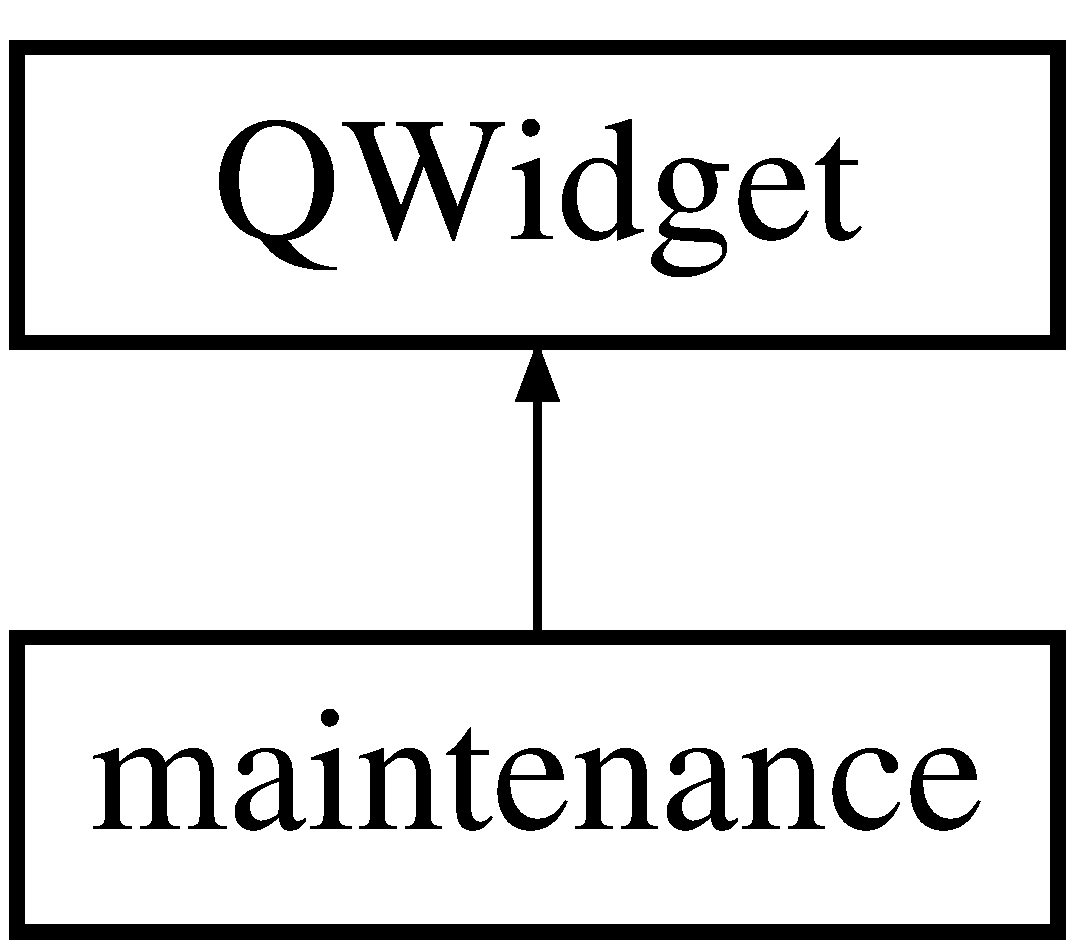
\includegraphics[height=2.000000cm]{classmaintenance}
\end{center}
\end{figure}
\subsection*{Public Member Functions}
\begin{DoxyCompactItemize}
\item 
\mbox{\hyperlink{classmaintenance_ae5cd12bbe9d483dd4d89123f52e31cf4}{maintenance}} (bool modifying=true, \mbox{\hyperlink{class_main_window}{Main\+Window}} $\ast$list\+Widget=0, \mbox{\hyperlink{structsouvenir_item}{souvenir\+Item}} souvenir=\mbox{\hyperlink{structsouvenir_item}{souvenir\+Item}}(), \mbox{\hyperlink{struct_college}{College}} college=\mbox{\hyperlink{struct_college}{College}}(), Q\+Widget $\ast$parent=0)
\begin{DoxyCompactList}\small\item\em \mbox{\hyperlink{classmaintenance_ae5cd12bbe9d483dd4d89123f52e31cf4}{maintenance\+::maintenance}} \end{DoxyCompactList}\item 
\mbox{\hyperlink{classmaintenance_a7d52b97e64d46d02e3365014d93e3148}{$\sim$maintenance}} ()
\begin{DoxyCompactList}\small\item\em \mbox{\hyperlink{classmaintenance_a7d52b97e64d46d02e3365014d93e3148}{maintenance\+::$\sim$maintenance}} \end{DoxyCompactList}\end{DoxyCompactItemize}


\subsection{Detailed Description}
The maintenance class This class will handle basic operations of User-\/\+Interface and altering database records used in the program. 

Maintenance Operations 

\subsection{Constructor \& Destructor Documentation}
\mbox{\Hypertarget{classmaintenance_ae5cd12bbe9d483dd4d89123f52e31cf4}\label{classmaintenance_ae5cd12bbe9d483dd4d89123f52e31cf4}} 
\index{maintenance@{maintenance}!maintenance@{maintenance}}
\index{maintenance@{maintenance}!maintenance@{maintenance}}
\subsubsection{\texorpdfstring{maintenance()}{maintenance()}}
{\footnotesize\ttfamily maintenance\+::maintenance (\begin{DoxyParamCaption}\item[{bool}]{modifying = {\ttfamily true},  }\item[{\mbox{\hyperlink{class_main_window}{Main\+Window}} $\ast$}]{main\+Window = {\ttfamily 0},  }\item[{\mbox{\hyperlink{structsouvenir_item}{souvenir\+Item}}}]{souvenir = {\ttfamily \mbox{\hyperlink{structsouvenir_item}{souvenir\+Item}}()},  }\item[{\mbox{\hyperlink{struct_college}{College}}}]{college = {\ttfamily \mbox{\hyperlink{struct_college}{College}}()},  }\item[{Q\+Widget $\ast$}]{parent = {\ttfamily 0} }\end{DoxyParamCaption})\hspace{0.3cm}{\ttfamily [explicit]}}



\mbox{\hyperlink{classmaintenance_ae5cd12bbe9d483dd4d89123f52e31cf4}{maintenance\+::maintenance}} 

Constructor 
\begin{DoxyParams}{Parameters}
{\em modifying} & -\/ bool if modifiying item \\
\hline
{\em main\+Window} & -\/ pointer to mainwindow for updates \\
\hline
{\em souvenir} & -\/ A struct argument \\
\hline
{\em college} & -\/ a struct argument \\
\hline
{\em parent} & \\
\hline
\end{DoxyParams}
\mbox{\Hypertarget{classmaintenance_a7d52b97e64d46d02e3365014d93e3148}\label{classmaintenance_a7d52b97e64d46d02e3365014d93e3148}} 
\index{maintenance@{maintenance}!````~maintenance@{$\sim$maintenance}}
\index{````~maintenance@{$\sim$maintenance}!maintenance@{maintenance}}
\subsubsection{\texorpdfstring{$\sim$maintenance()}{~maintenance()}}
{\footnotesize\ttfamily maintenance\+::$\sim$maintenance (\begin{DoxyParamCaption}{ }\end{DoxyParamCaption})}



\mbox{\hyperlink{classmaintenance_a7d52b97e64d46d02e3365014d93e3148}{maintenance\+::$\sim$maintenance}} 

Default Destructor 

The documentation for this class was generated from the following files\+:\begin{DoxyCompactItemize}
\item 
maintenance.\+h\item 
maintenance.\+cpp\end{DoxyCompactItemize}

\hypertarget{class_ui_1_1maintenance}{}\section{Ui\+:\+:maintenance Class Reference}
\label{class_ui_1_1maintenance}\index{Ui\+::maintenance@{Ui\+::maintenance}}
Inheritance diagram for Ui\+:\+:maintenance\+:\begin{figure}[H]
\begin{center}
\leavevmode
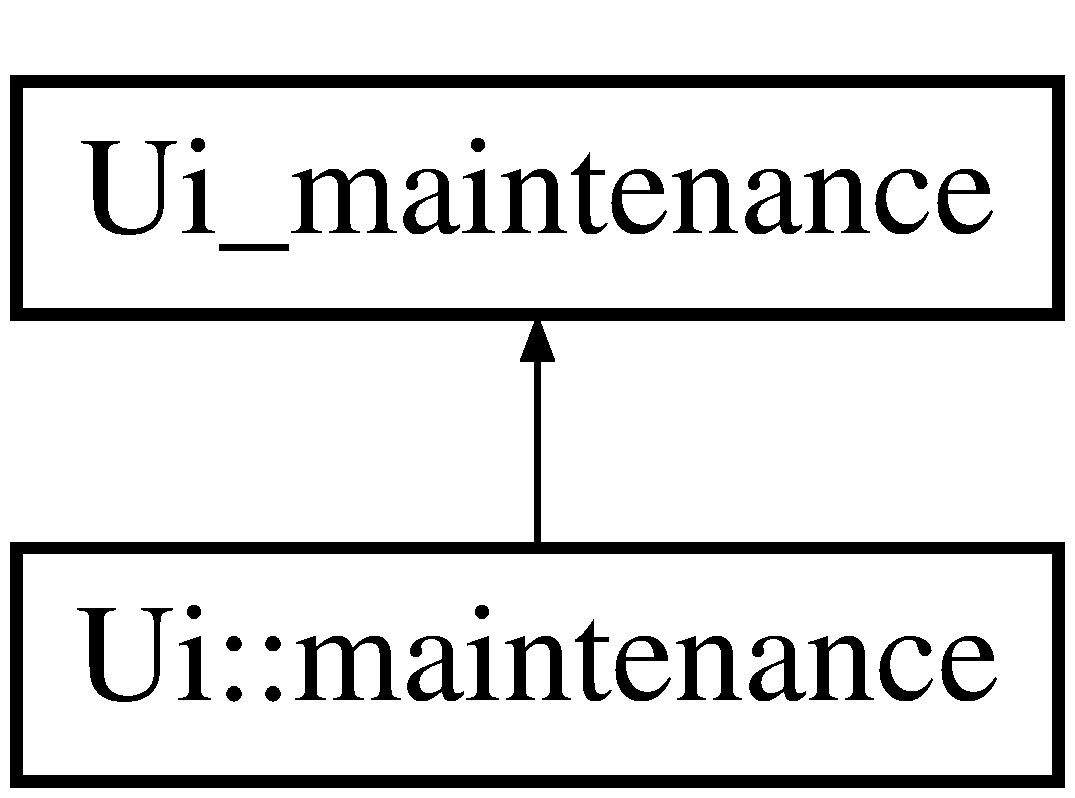
\includegraphics[height=2.000000cm]{class_ui_1_1maintenance}
\end{center}
\end{figure}
\subsection*{Additional Inherited Members}


The documentation for this class was generated from the following file\+:\begin{DoxyCompactItemize}
\item 
ui\+\_\+maintenance.\+h\end{DoxyCompactItemize}

\hypertarget{class_ui_1_1_main_window}{}\section{Ui\+:\+:Main\+Window Class Reference}
\label{class_ui_1_1_main_window}\index{Ui\+::\+Main\+Window@{Ui\+::\+Main\+Window}}
Inheritance diagram for Ui\+:\+:Main\+Window\+:\begin{figure}[H]
\begin{center}
\leavevmode
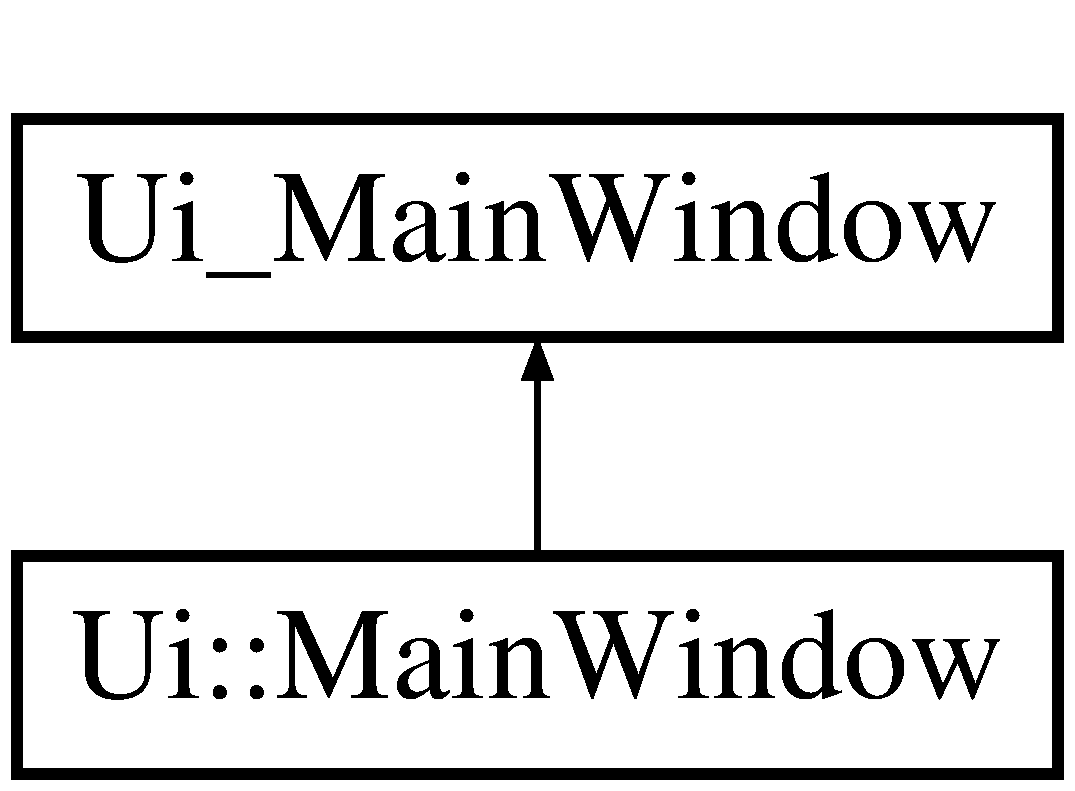
\includegraphics[height=2.000000cm]{class_ui_1_1_main_window}
\end{center}
\end{figure}
\subsection*{Additional Inherited Members}


The documentation for this class was generated from the following file\+:\begin{DoxyCompactItemize}
\item 
ui\+\_\+mainwindow.\+h\end{DoxyCompactItemize}

\hypertarget{class_main_window}{}\section{Main\+Window Class Reference}
\label{class_main_window}\index{Main\+Window@{Main\+Window}}
Inheritance diagram for Main\+Window\+:\begin{figure}[H]
\begin{center}
\leavevmode
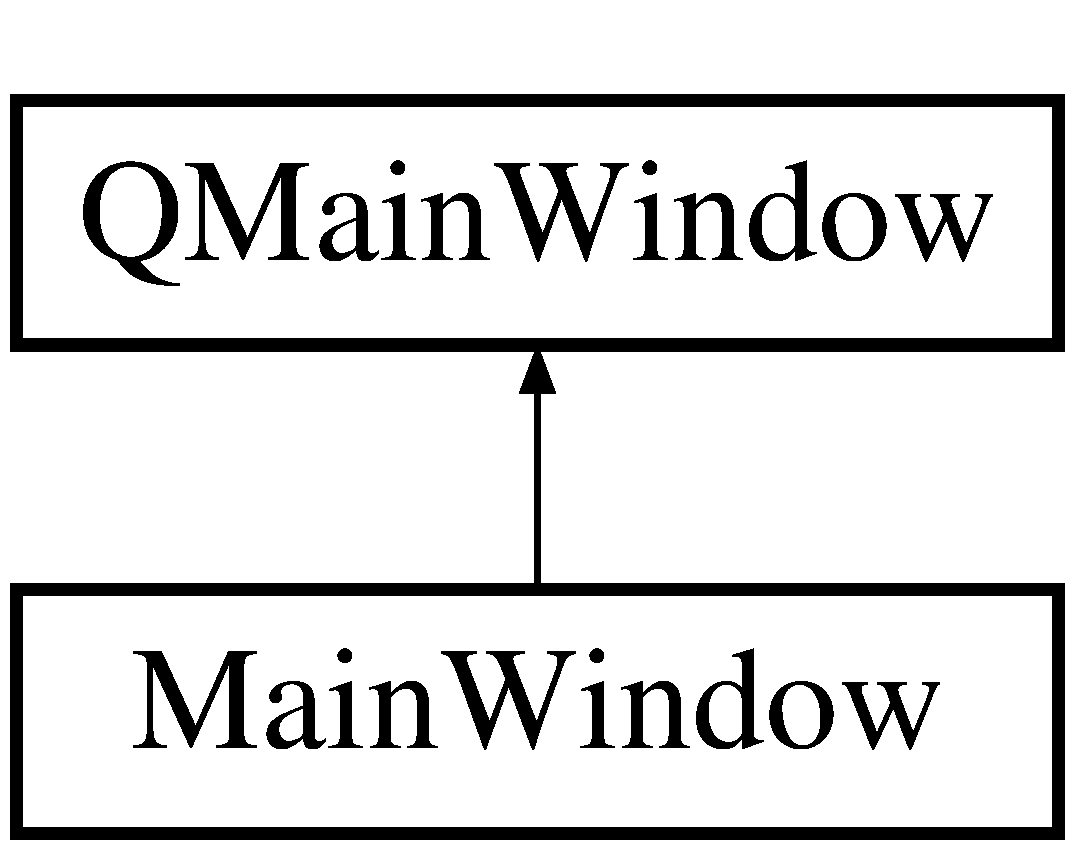
\includegraphics[height=2.000000cm]{class_main_window}
\end{center}
\end{figure}
\subsection*{Signals}
\begin{DoxyCompactItemize}
\item 
\mbox{\Hypertarget{class_main_window_ad176d91de00423f54f2d9eaabff52975}\label{class_main_window_ad176d91de00423f54f2d9eaabff52975}} 
void \mbox{\hyperlink{class_main_window_ad176d91de00423f54f2d9eaabff52975}{college\+Clicked\+Signal}} (\mbox{\hyperlink{struct_college}{College}})
\begin{DoxyCompactList}\small\item\em Default Destructor. \end{DoxyCompactList}\end{DoxyCompactItemize}
\subsection*{Public Member Functions}
\begin{DoxyCompactItemize}
\item 
\mbox{\Hypertarget{class_main_window_a8b244be8b7b7db1b08de2a2acb9409db}\label{class_main_window_a8b244be8b7b7db1b08de2a2acb9409db}} 
{\bfseries Main\+Window} (Q\+Widget $\ast$parent=0)
\item 
\mbox{\Hypertarget{class_main_window_ae253918de1b351d401c09856a6fef45a}\label{class_main_window_ae253918de1b351d401c09856a6fef45a}} 
void \mbox{\hyperlink{class_main_window_ae253918de1b351d401c09856a6fef45a}{populate\+Menu}} ()
\begin{DoxyCompactList}\small\item\em \mbox{\hyperlink{class_main_window_ae253918de1b351d401c09856a6fef45a}{Main\+Window\+::populate\+Menu}} Fills menu up with database colleges to allow user to choose which college they wish to start their custom trip at. \end{DoxyCompactList}\item 
void \mbox{\hyperlink{class_main_window_a8fd82811fcee5c9a13ea833a474950bb}{populate\+Admin\+Menu}} ()
\begin{DoxyCompactList}\small\item\em Populates main menu with colleges to start at. \end{DoxyCompactList}\item 
\mbox{\hyperlink{class_main_window_ae98d00a93bc118200eeef9f9bba1dba7}{$\sim$\+Main\+Window}} ()
\begin{DoxyCompactList}\small\item\em Populates admin menu with souvenirs from each college. \end{DoxyCompactList}\end{DoxyCompactItemize}


\subsection{Constructor \& Destructor Documentation}
\mbox{\Hypertarget{class_main_window_ae98d00a93bc118200eeef9f9bba1dba7}\label{class_main_window_ae98d00a93bc118200eeef9f9bba1dba7}} 
\index{Main\+Window@{Main\+Window}!````~Main\+Window@{$\sim$\+Main\+Window}}
\index{````~Main\+Window@{$\sim$\+Main\+Window}!Main\+Window@{Main\+Window}}
\subsubsection{\texorpdfstring{$\sim$\+Main\+Window()}{~MainWindow()}}
{\footnotesize\ttfamily Main\+Window\+::$\sim$\+Main\+Window (\begin{DoxyParamCaption}{ }\end{DoxyParamCaption})}



Populates admin menu with souvenirs from each college. 

\mbox{\hyperlink{class_main_window_ae98d00a93bc118200eeef9f9bba1dba7}{Main\+Window\+::$\sim$\+Main\+Window}}.

Default Destructor 

\subsection{Member Function Documentation}
\mbox{\Hypertarget{class_main_window_a8fd82811fcee5c9a13ea833a474950bb}\label{class_main_window_a8fd82811fcee5c9a13ea833a474950bb}} 
\index{Main\+Window@{Main\+Window}!populate\+Admin\+Menu@{populate\+Admin\+Menu}}
\index{populate\+Admin\+Menu@{populate\+Admin\+Menu}!Main\+Window@{Main\+Window}}
\subsubsection{\texorpdfstring{populate\+Admin\+Menu()}{populateAdminMenu()}}
{\footnotesize\ttfamily void Main\+Window\+::populate\+Admin\+Menu (\begin{DoxyParamCaption}{ }\end{DoxyParamCaption})}



Populates main menu with colleges to start at. 

\mbox{\hyperlink{class_main_window_a8fd82811fcee5c9a13ea833a474950bb}{Main\+Window\+::populate\+Admin\+Menu}} Populates admin menu with souvenir lists from which the user can select an item to change or delete. 

The documentation for this class was generated from the following files\+:\begin{DoxyCompactItemize}
\item 
mainwindow.\+h\item 
mainwindow.\+cpp\end{DoxyCompactItemize}

\hypertarget{structsouvenir_item}{}\section{souvenir\+Item Struct Reference}
\label{structsouvenir_item}\index{souvenir\+Item@{souvenir\+Item}}


The \mbox{\hyperlink{structsouvenir_item}{souvenir\+Item}} struct Will replicate details of a souvenir and will be composed into colleges to represent their souvenirs.  




{\ttfamily \#include $<$mainwindow.\+h$>$}

\subsection*{Public Attributes}
\begin{DoxyCompactItemize}
\item 
\mbox{\Hypertarget{structsouvenir_item_af15cfc3c9a9ad28a32c95c9eb9632e13}\label{structsouvenir_item_af15cfc3c9a9ad28a32c95c9eb9632e13}} 
int \mbox{\hyperlink{structsouvenir_item_af15cfc3c9a9ad28a32c95c9eb9632e13}{id}}
\begin{DoxyCompactList}\small\item\em The integer ID for each items. \end{DoxyCompactList}\item 
\mbox{\Hypertarget{structsouvenir_item_a39ed37d1f5d53285c8a7628c81946a13}\label{structsouvenir_item_a39ed37d1f5d53285c8a7628c81946a13}} 
Q\+String \mbox{\hyperlink{structsouvenir_item_a39ed37d1f5d53285c8a7628c81946a13}{name}}
\begin{DoxyCompactList}\small\item\em A Q\+String for the name of items. \end{DoxyCompactList}\item 
\mbox{\Hypertarget{structsouvenir_item_ab01bd33d7c6f6e716303eaf45cbc78fd}\label{structsouvenir_item_ab01bd33d7c6f6e716303eaf45cbc78fd}} 
double \mbox{\hyperlink{structsouvenir_item_ab01bd33d7c6f6e716303eaf45cbc78fd}{price}}
\begin{DoxyCompactList}\small\item\em A double to store each item\textquotesingle{}s price. \end{DoxyCompactList}\item 
\mbox{\Hypertarget{structsouvenir_item_a8a0c48f4b9b511e45e80fc21785469e9}\label{structsouvenir_item_a8a0c48f4b9b511e45e80fc21785469e9}} 
int \mbox{\hyperlink{structsouvenir_item_a8a0c48f4b9b511e45e80fc21785469e9}{quantity}}
\begin{DoxyCompactList}\small\item\em An integer to store quantity purchased. \end{DoxyCompactList}\end{DoxyCompactItemize}


\subsection{Detailed Description}
The \mbox{\hyperlink{structsouvenir_item}{souvenir\+Item}} struct Will replicate details of a souvenir and will be composed into colleges to represent their souvenirs. 

Souvenir Item Struct 

The documentation for this struct was generated from the following file\+:\begin{DoxyCompactItemize}
\item 
mainwindow.\+h\end{DoxyCompactItemize}

\hypertarget{class_ui_1_1totals}{}\section{Ui\+:\+:totals Class Reference}
\label{class_ui_1_1totals}\index{Ui\+::totals@{Ui\+::totals}}
Inheritance diagram for Ui\+:\+:totals\+:\begin{figure}[H]
\begin{center}
\leavevmode
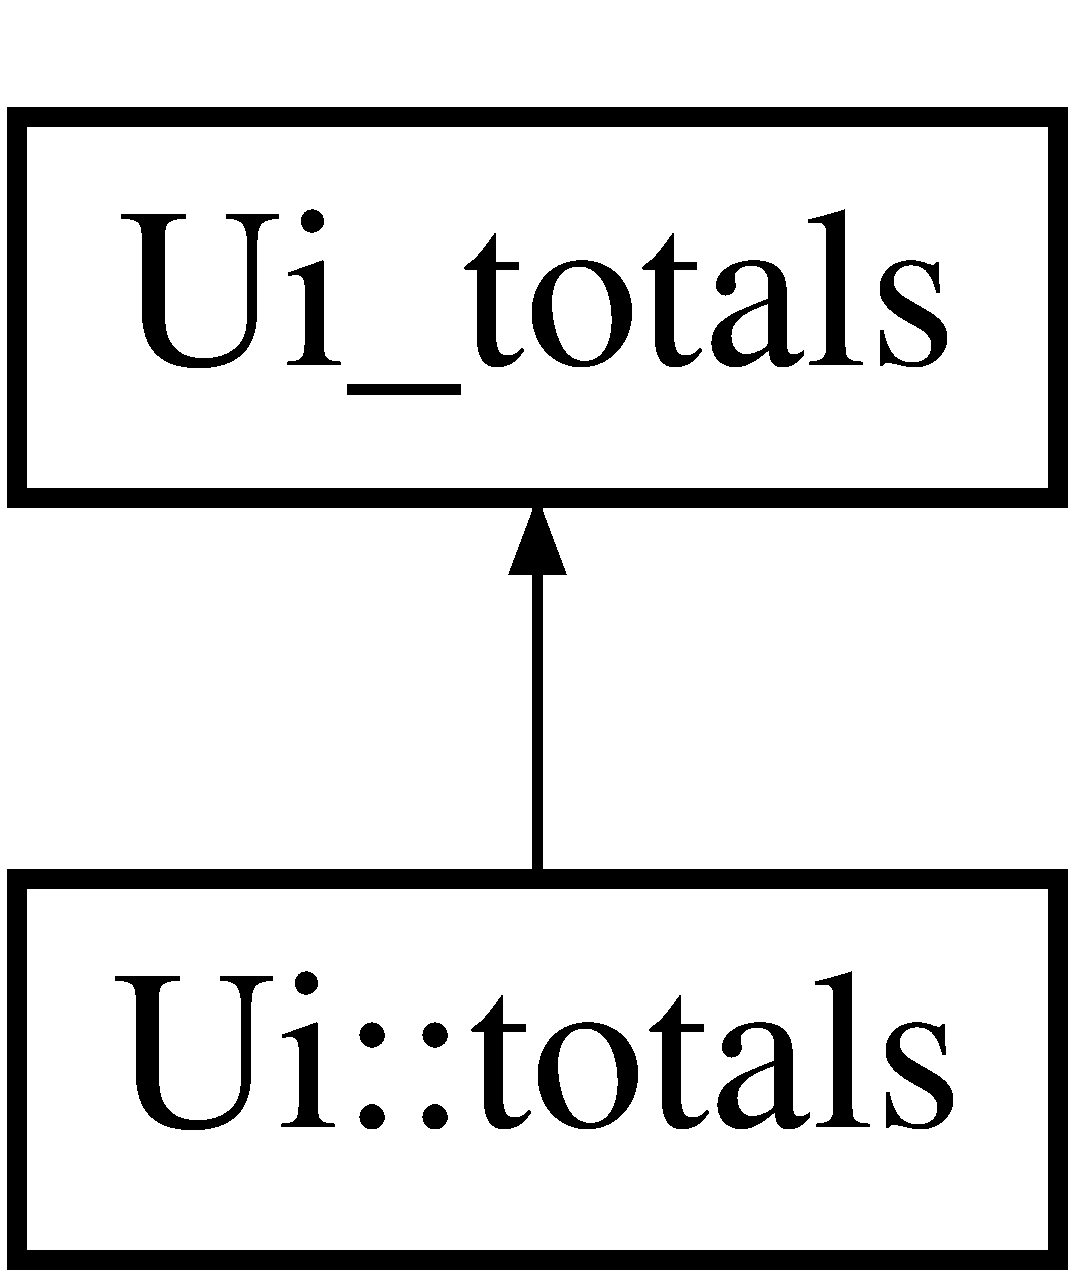
\includegraphics[height=2.000000cm]{class_ui_1_1totals}
\end{center}
\end{figure}
\subsection*{Additional Inherited Members}


The documentation for this class was generated from the following file\+:\begin{DoxyCompactItemize}
\item 
ui\+\_\+totals.\+h\end{DoxyCompactItemize}

\hypertarget{class_ui_1_1totals_sheet}{}\section{Ui\+:\+:totals\+Sheet Class Reference}
\label{class_ui_1_1totals_sheet}\index{Ui\+::totals\+Sheet@{Ui\+::totals\+Sheet}}
Inheritance diagram for Ui\+:\+:totals\+Sheet\+:\begin{figure}[H]
\begin{center}
\leavevmode
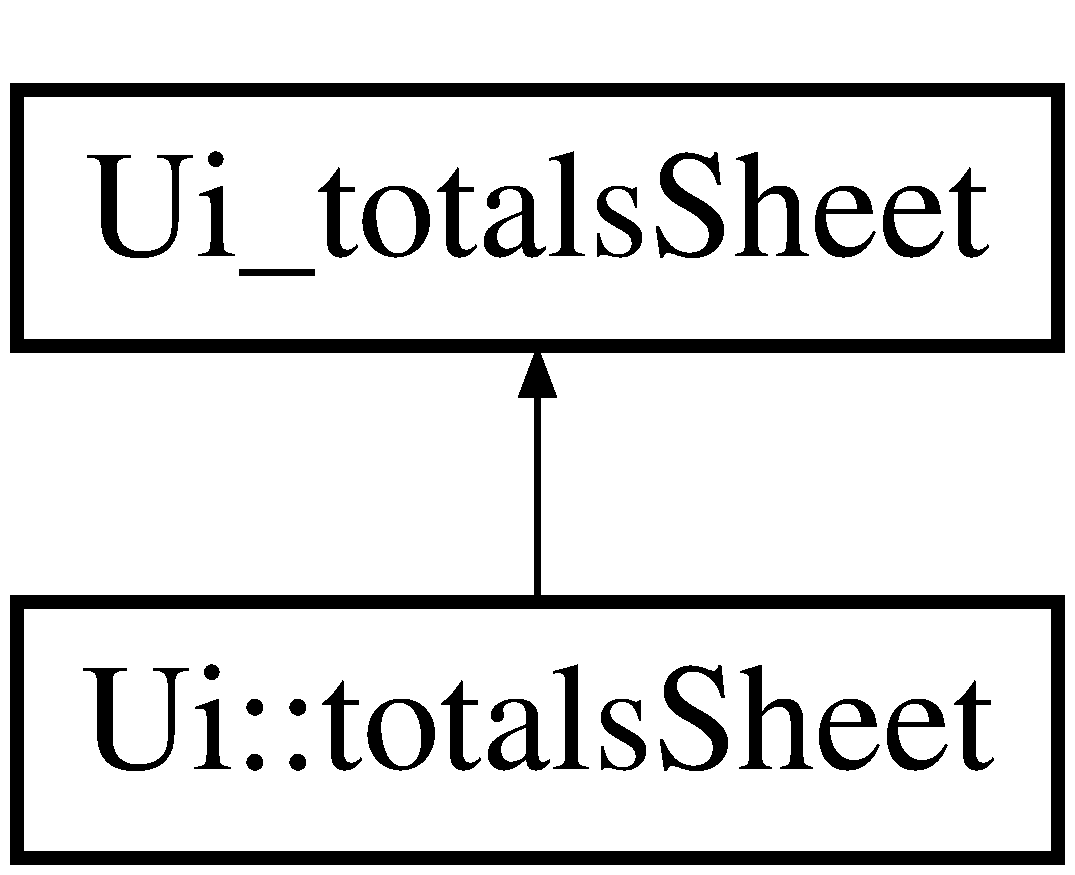
\includegraphics[height=2.000000cm]{class_ui_1_1totals_sheet}
\end{center}
\end{figure}
\subsection*{Additional Inherited Members}


The documentation for this class was generated from the following file\+:\begin{DoxyCompactItemize}
\item 
ui\+\_\+totalssheet.\+h\end{DoxyCompactItemize}

\hypertarget{classtotals_sheet}{}\section{totals\+Sheet Class Reference}
\label{classtotals_sheet}\index{totals\+Sheet@{totals\+Sheet}}


The \mbox{\hyperlink{classtotals_sheet}{totals\+Sheet}} class UI to display the expenses and invoice from the trip at the time it was invoked.  




{\ttfamily \#include $<$totalssheet.\+h$>$}

Inheritance diagram for totals\+Sheet\+:\begin{figure}[H]
\begin{center}
\leavevmode
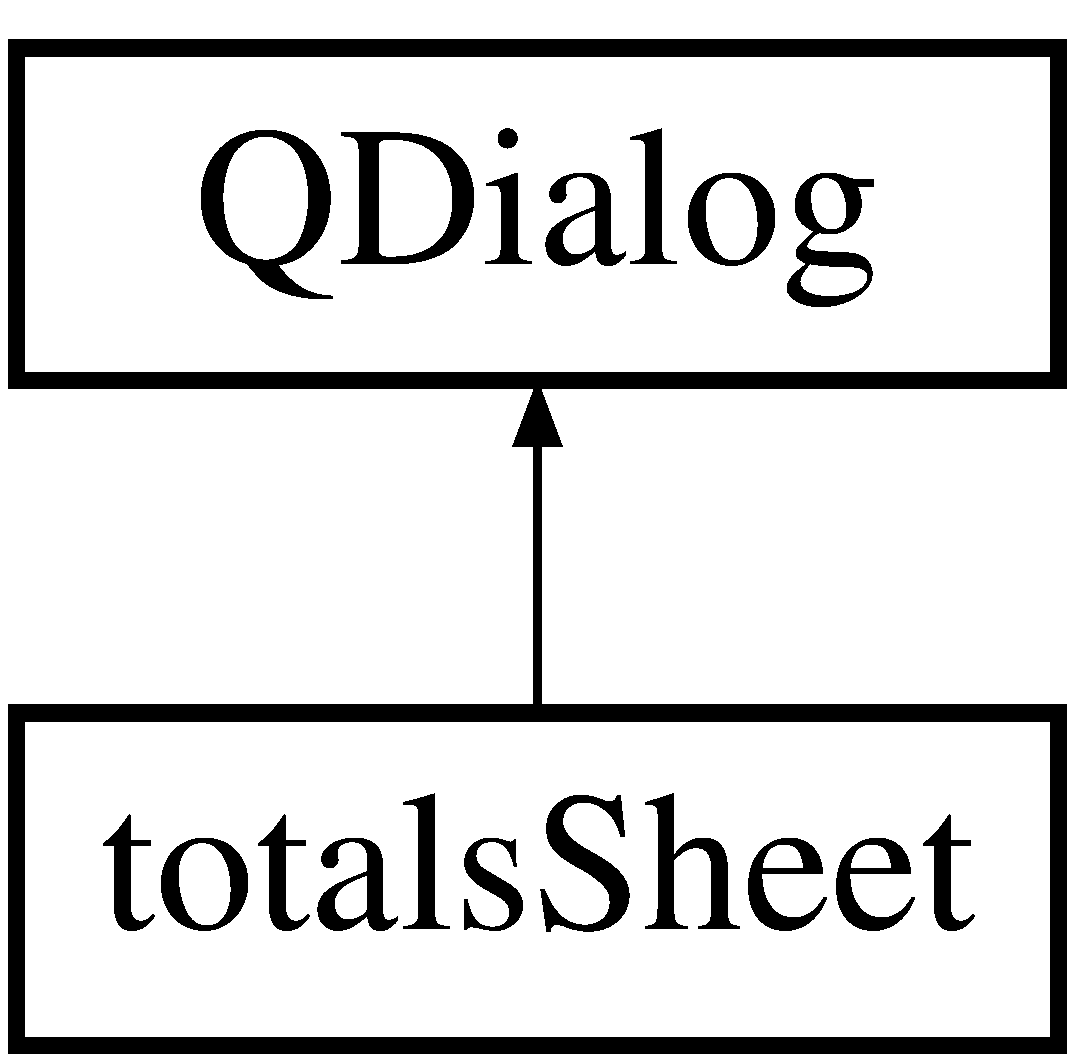
\includegraphics[height=2.000000cm]{classtotals_sheet}
\end{center}
\end{figure}
\subsection*{Public Member Functions}
\begin{DoxyCompactItemize}
\item 
\mbox{\hyperlink{classtotals_sheet_ab5b948f0b74c26fd822be62606d6ac35}{totals\+Sheet}} (\mbox{\hyperlink{class_cart}{Cart}} cart\+Info, Q\+Widget $\ast$parent=0)
\begin{DoxyCompactList}\small\item\em \mbox{\hyperlink{classtotals_sheet_ab5b948f0b74c26fd822be62606d6ac35}{totals\+Sheet\+::totals\+Sheet}} \end{DoxyCompactList}\item 
\mbox{\hyperlink{classtotals_sheet_a77d2ff4b0e0f02a4c05fbfa74bc6df84}{$\sim$totals\+Sheet}} ()
\begin{DoxyCompactList}\small\item\em Constructor. \end{DoxyCompactList}\end{DoxyCompactItemize}


\subsection{Detailed Description}
The \mbox{\hyperlink{classtotals_sheet}{totals\+Sheet}} class UI to display the expenses and invoice from the trip at the time it was invoked. 

Totals\+Sheet Class 

\subsection{Constructor \& Destructor Documentation}
\mbox{\Hypertarget{classtotals_sheet_ab5b948f0b74c26fd822be62606d6ac35}\label{classtotals_sheet_ab5b948f0b74c26fd822be62606d6ac35}} 
\index{totals\+Sheet@{totals\+Sheet}!totals\+Sheet@{totals\+Sheet}}
\index{totals\+Sheet@{totals\+Sheet}!totals\+Sheet@{totals\+Sheet}}
\subsubsection{\texorpdfstring{totals\+Sheet()}{totalsSheet()}}
{\footnotesize\ttfamily totals\+Sheet\+::totals\+Sheet (\begin{DoxyParamCaption}\item[{\mbox{\hyperlink{class_cart}{Cart}}}]{cart\+Info,  }\item[{Q\+Widget $\ast$}]{parent = {\ttfamily 0} }\end{DoxyParamCaption})\hspace{0.3cm}{\ttfamily [explicit]}}



\mbox{\hyperlink{classtotals_sheet_ab5b948f0b74c26fd822be62606d6ac35}{totals\+Sheet\+::totals\+Sheet}} 

Constructor 
\begin{DoxyParams}{Parameters}
{\em cart\+Info} & -\/ A class argument \\
\hline
{\em parent} & \\
\hline
\end{DoxyParams}
\mbox{\Hypertarget{classtotals_sheet_a77d2ff4b0e0f02a4c05fbfa74bc6df84}\label{classtotals_sheet_a77d2ff4b0e0f02a4c05fbfa74bc6df84}} 
\index{totals\+Sheet@{totals\+Sheet}!````~totals\+Sheet@{$\sim$totals\+Sheet}}
\index{````~totals\+Sheet@{$\sim$totals\+Sheet}!totals\+Sheet@{totals\+Sheet}}
\subsubsection{\texorpdfstring{$\sim$totals\+Sheet()}{~totalsSheet()}}
{\footnotesize\ttfamily totals\+Sheet\+::$\sim$totals\+Sheet (\begin{DoxyParamCaption}{ }\end{DoxyParamCaption})}



Constructor. 

\mbox{\hyperlink{classtotals_sheet_a77d2ff4b0e0f02a4c05fbfa74bc6df84}{totals\+Sheet\+::$\sim$totals\+Sheet}}

Destructor 

The documentation for this class was generated from the following files\+:\begin{DoxyCompactItemize}
\item 
totalssheet.\+h\item 
totalssheet.\+cpp\end{DoxyCompactItemize}

\hypertarget{class_transaction}{}\section{Transaction Class Reference}
\label{class_transaction}\index{Transaction@{Transaction}}


The \mbox{\hyperlink{class_transaction}{Transaction}} class.  




{\ttfamily \#include $<$cart.\+h$>$}

\subsection*{Public Member Functions}
\begin{DoxyCompactItemize}
\item 
bool \mbox{\hyperlink{class_transaction_af91c48f0072425f2c65cb3689ca6c653}{operator==}} (\mbox{\hyperlink{class_transaction}{Transaction}} \&other)
\begin{DoxyCompactList}\small\item\em Overloaded Operator. \end{DoxyCompactList}\item 
\mbox{\hyperlink{class_transaction_a027ee3210228e05081452160100a65df}{Transaction}} (\mbox{\hyperlink{struct_college}{College}} \mbox{\hyperlink{class_transaction_a8789961780bef7d71a64eb894fb57d84}{college}}, \mbox{\hyperlink{structsouvenir_item}{souvenir\+Item}} \mbox{\hyperlink{class_transaction_a2526fe971714943e90457cc9bce61b56}{item\+Purchased}})
\begin{DoxyCompactList}\small\item\em A Constructor. \end{DoxyCompactList}\item 
\mbox{\Hypertarget{class_transaction_ab47005b855d38bc324bb79fd023baa13}\label{class_transaction_ab47005b855d38bc324bb79fd023baa13}} 
\mbox{\hyperlink{class_transaction_ab47005b855d38bc324bb79fd023baa13}{Transaction}} ()
\begin{DoxyCompactList}\small\item\em Default Constructor. \end{DoxyCompactList}\item 
\mbox{\Hypertarget{class_transaction_a362b0d2524d0c799165190517192dca9}\label{class_transaction_a362b0d2524d0c799165190517192dca9}} 
\mbox{\hyperlink{class_transaction_a362b0d2524d0c799165190517192dca9}{$\sim$\+Transaction}} ()
\begin{DoxyCompactList}\small\item\em Default Constructor. \end{DoxyCompactList}\end{DoxyCompactItemize}
\subsection*{Public Attributes}
\begin{DoxyCompactItemize}
\item 
\mbox{\Hypertarget{class_transaction_a8789961780bef7d71a64eb894fb57d84}\label{class_transaction_a8789961780bef7d71a64eb894fb57d84}} 
\mbox{\hyperlink{struct_college}{College}} \mbox{\hyperlink{class_transaction_a8789961780bef7d71a64eb894fb57d84}{college}}
\begin{DoxyCompactList}\small\item\em Struct of college to represent colleges. \end{DoxyCompactList}\item 
\mbox{\Hypertarget{class_transaction_a2526fe971714943e90457cc9bce61b56}\label{class_transaction_a2526fe971714943e90457cc9bce61b56}} 
\mbox{\hyperlink{structsouvenir_item}{souvenir\+Item}} \mbox{\hyperlink{class_transaction_a2526fe971714943e90457cc9bce61b56}{item\+Purchased}}
\begin{DoxyCompactList}\small\item\em Struct of souvenir items to track purchasing. \end{DoxyCompactList}\end{DoxyCompactItemize}


\subsection{Detailed Description}
The \mbox{\hyperlink{class_transaction}{Transaction}} class. 

The \mbox{\hyperlink{class_transaction}{Transaction}} Handler The transaction class will handle operations in the cart class of which it is composed as a private Q\+Vector data member. 

\subsection{Constructor \& Destructor Documentation}
\mbox{\Hypertarget{class_transaction_a027ee3210228e05081452160100a65df}\label{class_transaction_a027ee3210228e05081452160100a65df}} 
\index{Transaction@{Transaction}!Transaction@{Transaction}}
\index{Transaction@{Transaction}!Transaction@{Transaction}}
\subsubsection{\texorpdfstring{Transaction()}{Transaction()}}
{\footnotesize\ttfamily Transaction\+::\+Transaction (\begin{DoxyParamCaption}\item[{\mbox{\hyperlink{struct_college}{College}}}]{college,  }\item[{\mbox{\hyperlink{structsouvenir_item}{souvenir\+Item}}}]{item\+Purchased }\end{DoxyParamCaption})}



A Constructor. 

\mbox{\hyperlink{class_transaction_a027ee3210228e05081452160100a65df}{Transaction\+::\+Transaction}}.

\mbox{\hyperlink{class_transaction}{Transaction}} Sets the arguments that are passed into the classes data members. 
\begin{DoxyParams}{Parameters}
{\em college} & -\/ A struct argument \\
\hline
{\em item\+Purchased} & -\/ A struct argument\\
\hline
\end{DoxyParams}
Constructor with parameters 
\begin{DoxyParams}{Parameters}
{\em college} & -\/ A struct argument \\
\hline
{\em item\+Purchased} & -\/ A struct argument \\
\hline
\end{DoxyParams}


\subsection{Member Function Documentation}
\mbox{\Hypertarget{class_transaction_af91c48f0072425f2c65cb3689ca6c653}\label{class_transaction_af91c48f0072425f2c65cb3689ca6c653}} 
\index{Transaction@{Transaction}!operator==@{operator==}}
\index{operator==@{operator==}!Transaction@{Transaction}}
\subsubsection{\texorpdfstring{operator==()}{operator==()}}
{\footnotesize\ttfamily bool Transaction\+::operator== (\begin{DoxyParamCaption}\item[{\mbox{\hyperlink{class_transaction}{Transaction}} \&}]{other }\end{DoxyParamCaption})}



Overloaded Operator. 

\mbox{\hyperlink{class_transaction_af91c48f0072425f2c65cb3689ca6c653}{Transaction\+::operator ==}}.

operator == Overloads the \textquotesingle{}equal to\textquotesingle{} operator for processing 
\begin{DoxyParams}{Parameters}
{\em other} & the items purchased to be compared for reassurance of correct item \\
\hline
\end{DoxyParams}
\begin{DoxyReturn}{Returns}
A boolean that is true if this item is equal to the other item
\end{DoxyReturn}
Overloaded Operator 
\begin{DoxyParams}{Parameters}
{\em other} & -\/ A class argument \\
\hline
\end{DoxyParams}
\begin{DoxyReturn}{Returns}
boolean for if they are equivalent or not 
\end{DoxyReturn}


The documentation for this class was generated from the following files\+:\begin{DoxyCompactItemize}
\item 
cart.\+h\item 
cart.\+cpp\end{DoxyCompactItemize}

\hypertarget{class_ui___college_model}{}\section{Ui\+\_\+\+College\+Model Class Reference}
\label{class_ui___college_model}\index{Ui\+\_\+\+College\+Model@{Ui\+\_\+\+College\+Model}}
Inheritance diagram for Ui\+\_\+\+College\+Model\+:\begin{figure}[H]
\begin{center}
\leavevmode
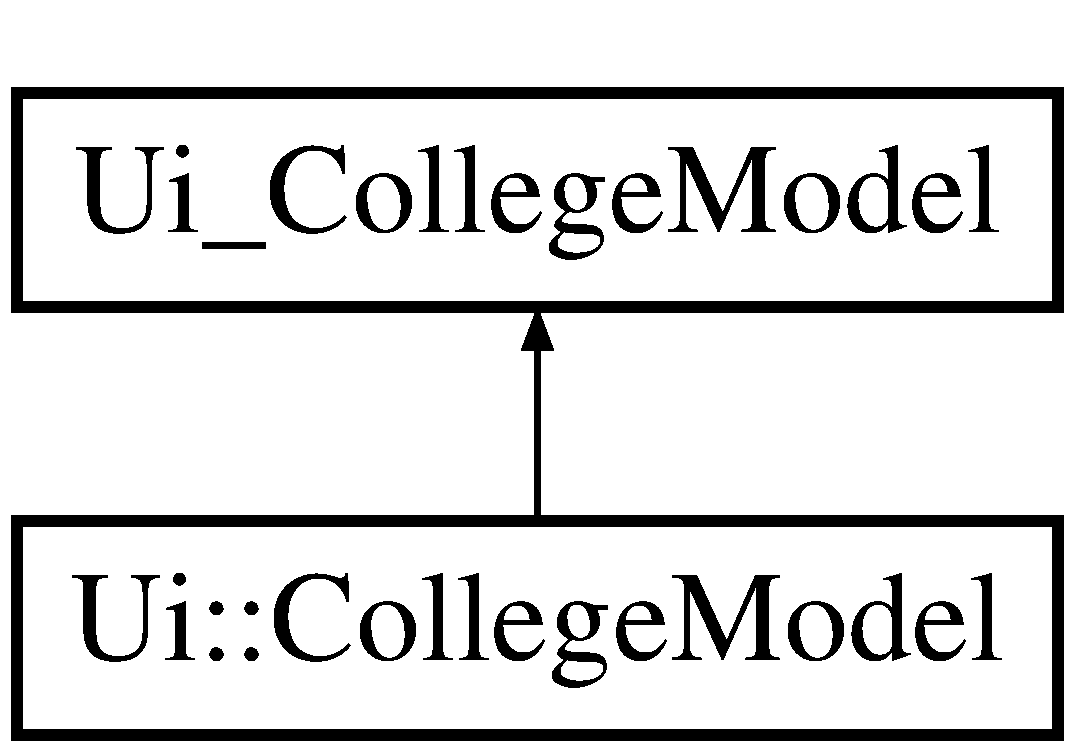
\includegraphics[height=2.000000cm]{class_ui___college_model}
\end{center}
\end{figure}
\subsection*{Public Member Functions}
\begin{DoxyCompactItemize}
\item 
\mbox{\Hypertarget{class_ui___college_model_ab7cc17baa43b5458dacf9d3709b4078e}\label{class_ui___college_model_ab7cc17baa43b5458dacf9d3709b4078e}} 
void {\bfseries setup\+Ui} (Q\+Widget $\ast$\mbox{\hyperlink{class_college_model}{College\+Model}})
\item 
\mbox{\Hypertarget{class_ui___college_model_ab6aac2770d1344acccf8aab4858011e4}\label{class_ui___college_model_ab6aac2770d1344acccf8aab4858011e4}} 
void {\bfseries retranslate\+Ui} (Q\+Widget $\ast$\mbox{\hyperlink{class_college_model}{College\+Model}})
\end{DoxyCompactItemize}
\subsection*{Public Attributes}
\begin{DoxyCompactItemize}
\item 
\mbox{\Hypertarget{class_ui___college_model_a5e12a43e4b076638884cb3a9b6fa5829}\label{class_ui___college_model_a5e12a43e4b076638884cb3a9b6fa5829}} 
Q\+Stacked\+Widget $\ast$ {\bfseries college\+\_\+model\+\_\+stacked\+\_\+widget}
\item 
\mbox{\Hypertarget{class_ui___college_model_aa888e05de98f70d3e671b9f3dd756341}\label{class_ui___college_model_aa888e05de98f70d3e671b9f3dd756341}} 
Q\+Widget $\ast$ {\bfseries trip\+\_\+page}
\item 
\mbox{\Hypertarget{class_ui___college_model_a855d636108b9966f9dba7af960afae12}\label{class_ui___college_model_a855d636108b9966f9dba7af960afae12}} 
Q\+Push\+Button $\ast$ {\bfseries next\+\_\+college\+\_\+button}
\item 
\mbox{\Hypertarget{class_ui___college_model_aeb428c3b9e1441a8dd583990a9276ac6}\label{class_ui___college_model_aeb428c3b9e1441a8dd583990a9276ac6}} 
Q\+Group\+Box $\ast$ {\bfseries souvenir\+\_\+group\+\_\+box}
\item 
\mbox{\Hypertarget{class_ui___college_model_afddeae1cc8ee19be345846e7ed232fa6}\label{class_ui___college_model_afddeae1cc8ee19be345846e7ed232fa6}} 
Q\+Widget $\ast$ {\bfseries vertical\+Layout\+Widget}
\item 
\mbox{\Hypertarget{class_ui___college_model_a09de040d3b700cc0085f868212520549}\label{class_ui___college_model_a09de040d3b700cc0085f868212520549}} 
Q\+V\+Box\+Layout $\ast$ {\bfseries vertical\+Layout}
\item 
\mbox{\Hypertarget{class_ui___college_model_aae99167d3e36075850253e42bf517a87}\label{class_ui___college_model_aae99167d3e36075850253e42bf517a87}} 
Q\+Grid\+Layout $\ast$ {\bfseries grid\+Layout}
\item 
\mbox{\Hypertarget{class_ui___college_model_a50f9c221f77d276514e53080dac0e3b5}\label{class_ui___college_model_a50f9c221f77d276514e53080dac0e3b5}} 
Q\+Label $\ast$ {\bfseries trip\+\_\+distance\+\_\+label}
\item 
\mbox{\Hypertarget{class_ui___college_model_aad4c78b139b0ad7a529fb521fff62493}\label{class_ui___college_model_aad4c78b139b0ad7a529fb521fff62493}} 
Q\+Widget $\ast$ {\bfseries layout\+Widget}
\item 
\mbox{\Hypertarget{class_ui___college_model_af7e7adfc112d0cad9cd8976c33beab42}\label{class_ui___college_model_af7e7adfc112d0cad9cd8976c33beab42}} 
Q\+V\+Box\+Layout $\ast$ {\bfseries vertical\+Layout\+\_\+2}
\item 
\mbox{\Hypertarget{class_ui___college_model_a2c1d77a412a2b9cb95f7115d9829960b}\label{class_ui___college_model_a2c1d77a412a2b9cb95f7115d9829960b}} 
Q\+Label $\ast$ {\bfseries totals\+\_\+label}
\item 
\mbox{\Hypertarget{class_ui___college_model_a3812bc4f1708ddade3eaf6e66689bac3}\label{class_ui___college_model_a3812bc4f1708ddade3eaf6e66689bac3}} 
Q\+Push\+Button $\ast$ {\bfseries totals\+\_\+button}
\item 
\mbox{\Hypertarget{class_ui___college_model_a17a6d8122d50896b30bb85830761e6d1}\label{class_ui___college_model_a17a6d8122d50896b30bb85830761e6d1}} 
Q\+Widget $\ast$ {\bfseries layout\+Widget1}
\item 
\mbox{\Hypertarget{class_ui___college_model_a4e4dd1b75828e4855b92cad3560fcae6}\label{class_ui___college_model_a4e4dd1b75828e4855b92cad3560fcae6}} 
Q\+H\+Box\+Layout $\ast$ {\bfseries horizontal\+Layout\+\_\+5}
\item 
\mbox{\Hypertarget{class_ui___college_model_ae2cd3354c4e9c980a8959b5437b0a119}\label{class_ui___college_model_ae2cd3354c4e9c980a8959b5437b0a119}} 
Q\+Frame $\ast$ {\bfseries line\+\_\+5}
\item 
\mbox{\Hypertarget{class_ui___college_model_ad05dfa256c775a4b29f294f5d22c6efa}\label{class_ui___college_model_ad05dfa256c775a4b29f294f5d22c6efa}} 
Q\+Label $\ast$ {\bfseries college\+\_\+name\+\_\+label}
\item 
\mbox{\Hypertarget{class_ui___college_model_ad76fab19c01dcc14616c6d14f54cc3d4}\label{class_ui___college_model_ad76fab19c01dcc14616c6d14f54cc3d4}} 
Q\+Frame $\ast$ {\bfseries line\+\_\+6}
\item 
\mbox{\Hypertarget{class_ui___college_model_ab8e3a51ed4e61b355d58c4ffa0e4fc32}\label{class_ui___college_model_ab8e3a51ed4e61b355d58c4ffa0e4fc32}} 
Q\+Widget $\ast$ {\bfseries layout\+Widget2}
\item 
\mbox{\Hypertarget{class_ui___college_model_a4a26d7ef7985c3afe7edf8d44993060d}\label{class_ui___college_model_a4a26d7ef7985c3afe7edf8d44993060d}} 
Q\+V\+Box\+Layout $\ast$ {\bfseries vertical\+Layout\+\_\+3}
\item 
\mbox{\Hypertarget{class_ui___college_model_ab114774778a03d391b8fdb686d2ff010}\label{class_ui___college_model_ab114774778a03d391b8fdb686d2ff010}} 
Q\+List\+Widget $\ast$ {\bfseries cart\+List}
\item 
\mbox{\Hypertarget{class_ui___college_model_a4678c72de2b36f9e4c2bf67c5295db2e}\label{class_ui___college_model_a4678c72de2b36f9e4c2bf67c5295db2e}} 
Q\+H\+Box\+Layout $\ast$ {\bfseries horizontal\+Layout}
\item 
\mbox{\Hypertarget{class_ui___college_model_ad95dfaa4d3fa5fab98def86ca67dff97}\label{class_ui___college_model_ad95dfaa4d3fa5fab98def86ca67dff97}} 
Q\+Spacer\+Item $\ast$ {\bfseries horizontal\+Spacer}
\item 
\mbox{\Hypertarget{class_ui___college_model_a630aa984876af90fb90f2a21bdcfb91d}\label{class_ui___college_model_a630aa984876af90fb90f2a21bdcfb91d}} 
Q\+Push\+Button $\ast$ {\bfseries remove\+Cart\+Item\+Button}
\item 
\mbox{\Hypertarget{class_ui___college_model_a9393559266eb04e033fb73de60fc5dfb}\label{class_ui___college_model_a9393559266eb04e033fb73de60fc5dfb}} 
Q\+Spacer\+Item $\ast$ {\bfseries horizontal\+Spacer\+\_\+2}
\item 
\mbox{\Hypertarget{class_ui___college_model_a3241dfbe29d6991f780bade76e1e0cce}\label{class_ui___college_model_a3241dfbe29d6991f780bade76e1e0cce}} 
Q\+Widget $\ast$ {\bfseries loading\+\_\+page}
\item 
\mbox{\Hypertarget{class_ui___college_model_aafae2091bfa9eedc53b46eb30dde542f}\label{class_ui___college_model_aafae2091bfa9eedc53b46eb30dde542f}} 
Q\+Widget $\ast$ {\bfseries layout\+Widget3}
\item 
\mbox{\Hypertarget{class_ui___college_model_a92a71bea4f774afd0c11071abf06ba10}\label{class_ui___college_model_a92a71bea4f774afd0c11071abf06ba10}} 
Q\+H\+Box\+Layout $\ast$ {\bfseries horizontal\+Layout\+\_\+3}
\item 
\mbox{\Hypertarget{class_ui___college_model_a6a4c9ccff9a8838f37ebfbec8fffe656}\label{class_ui___college_model_a6a4c9ccff9a8838f37ebfbec8fffe656}} 
Q\+Frame $\ast$ {\bfseries line}
\item 
\mbox{\Hypertarget{class_ui___college_model_a1c7027b62487286b5f425473a292873e}\label{class_ui___college_model_a1c7027b62487286b5f425473a292873e}} 
Q\+Spacer\+Item $\ast$ {\bfseries horizontal\+Spacer\+\_\+5}
\item 
\mbox{\Hypertarget{class_ui___college_model_a4f9c9dda155fa0f96b30a19b4ce16eb8}\label{class_ui___college_model_a4f9c9dda155fa0f96b30a19b4ce16eb8}} 
Q\+Label $\ast$ {\bfseries loading\+\_\+gif}
\item 
\mbox{\Hypertarget{class_ui___college_model_a1c53332578941723723d638ce943f46f}\label{class_ui___college_model_a1c53332578941723723d638ce943f46f}} 
Q\+Spacer\+Item $\ast$ {\bfseries horizontal\+Spacer\+\_\+6}
\item 
\mbox{\Hypertarget{class_ui___college_model_a57800ea6f890bc6a99bcc4a0f164c2a8}\label{class_ui___college_model_a57800ea6f890bc6a99bcc4a0f164c2a8}} 
Q\+Frame $\ast$ {\bfseries line\+\_\+2}
\item 
\mbox{\Hypertarget{class_ui___college_model_a1dc907e4b7248cc743c968dc1e61148c}\label{class_ui___college_model_a1dc907e4b7248cc743c968dc1e61148c}} 
Q\+Widget $\ast$ {\bfseries layout\+Widget4}
\item 
\mbox{\Hypertarget{class_ui___college_model_adbfb72e4580306a4877230ce3edb7098}\label{class_ui___college_model_adbfb72e4580306a4877230ce3edb7098}} 
Q\+H\+Box\+Layout $\ast$ {\bfseries horizontal\+Layout\+\_\+4}
\item 
\mbox{\Hypertarget{class_ui___college_model_a3cba7f7dfe5b984ab0a7a38b6884cd55}\label{class_ui___college_model_a3cba7f7dfe5b984ab0a7a38b6884cd55}} 
Q\+Frame $\ast$ {\bfseries line\+\_\+3}
\item 
\mbox{\Hypertarget{class_ui___college_model_afafb10cd25d6e9f4350677130193512b}\label{class_ui___college_model_afafb10cd25d6e9f4350677130193512b}} 
Q\+H\+Box\+Layout $\ast$ {\bfseries horizontal\+Layout\+\_\+2}
\item 
\mbox{\Hypertarget{class_ui___college_model_a4a6598ce1fd4560615ca94872dbc7f3c}\label{class_ui___college_model_a4a6598ce1fd4560615ca94872dbc7f3c}} 
Q\+Spacer\+Item $\ast$ {\bfseries horizontal\+Spacer\+\_\+3}
\item 
\mbox{\Hypertarget{class_ui___college_model_a61047000346207cced67e38e1d94603f}\label{class_ui___college_model_a61047000346207cced67e38e1d94603f}} 
Q\+Label $\ast$ {\bfseries loading\+\_\+label}
\item 
\mbox{\Hypertarget{class_ui___college_model_afa37370f8db338cac2ee6ca71c3cffdc}\label{class_ui___college_model_afa37370f8db338cac2ee6ca71c3cffdc}} 
Q\+Spacer\+Item $\ast$ {\bfseries horizontal\+Spacer\+\_\+4}
\item 
\mbox{\Hypertarget{class_ui___college_model_a6e0b9090a33af7a4b3db31a9bcf81a85}\label{class_ui___college_model_a6e0b9090a33af7a4b3db31a9bcf81a85}} 
Q\+Frame $\ast$ {\bfseries line\+\_\+4}
\end{DoxyCompactItemize}


The documentation for this class was generated from the following file\+:\begin{DoxyCompactItemize}
\item 
ui\+\_\+collegemodel.\+h\end{DoxyCompactItemize}

\hypertarget{class_ui__maintenance}{}\section{Ui\+\_\+maintenance Class Reference}
\label{class_ui__maintenance}\index{Ui\+\_\+maintenance@{Ui\+\_\+maintenance}}
Inheritance diagram for Ui\+\_\+maintenance\+:\begin{figure}[H]
\begin{center}
\leavevmode
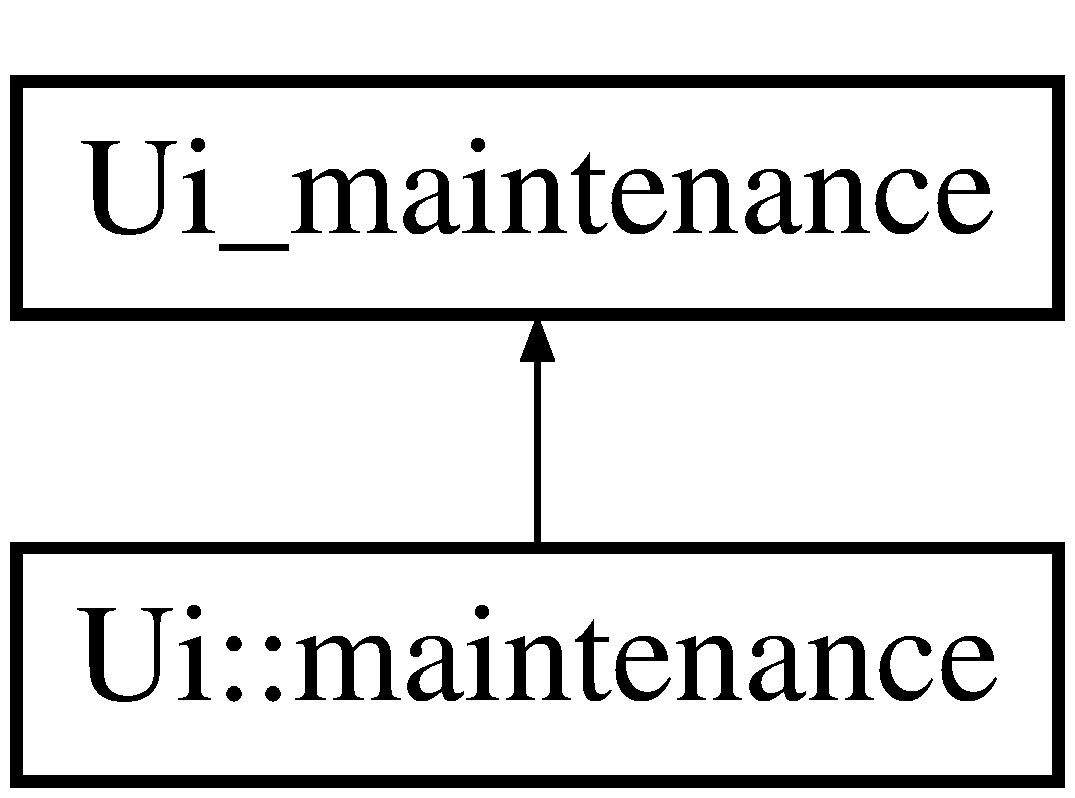
\includegraphics[height=2.000000cm]{class_ui__maintenance}
\end{center}
\end{figure}
\subsection*{Public Member Functions}
\begin{DoxyCompactItemize}
\item 
\mbox{\Hypertarget{class_ui__maintenance_a664c5b70f69f736c4607afa83106c54d}\label{class_ui__maintenance_a664c5b70f69f736c4607afa83106c54d}} 
void {\bfseries setup\+Ui} (Q\+Widget $\ast$\mbox{\hyperlink{classmaintenance}{maintenance}})
\item 
\mbox{\Hypertarget{class_ui__maintenance_a488b009956e9bc6bb32e67aca9de7a2b}\label{class_ui__maintenance_a488b009956e9bc6bb32e67aca9de7a2b}} 
void {\bfseries retranslate\+Ui} (Q\+Widget $\ast$\mbox{\hyperlink{classmaintenance}{maintenance}})
\end{DoxyCompactItemize}
\subsection*{Public Attributes}
\begin{DoxyCompactItemize}
\item 
\mbox{\Hypertarget{class_ui__maintenance_ad11afee85bdcb2af776a3dd4766bec7b}\label{class_ui__maintenance_ad11afee85bdcb2af776a3dd4766bec7b}} 
Q\+Grid\+Layout $\ast$ {\bfseries grid\+Layout\+\_\+4}
\item 
\mbox{\Hypertarget{class_ui__maintenance_afb9597d153d8f5390d8e93396c765800}\label{class_ui__maintenance_afb9597d153d8f5390d8e93396c765800}} 
Q\+Stacked\+Widget $\ast$ {\bfseries maintenance\+\_\+stacked\+\_\+widget}
\item 
\mbox{\Hypertarget{class_ui__maintenance_aa8cb8f7076cb9afddf2f7fb39117cf3f}\label{class_ui__maintenance_aa8cb8f7076cb9afddf2f7fb39117cf3f}} 
Q\+Widget $\ast$ {\bfseries add\+\_\+item\+\_\+page}
\item 
\mbox{\Hypertarget{class_ui__maintenance_a1ff9a605a3105ee1bf6d709ecdfd3754}\label{class_ui__maintenance_a1ff9a605a3105ee1bf6d709ecdfd3754}} 
Q\+Grid\+Layout $\ast$ {\bfseries grid\+Layout\+\_\+2}
\item 
\mbox{\Hypertarget{class_ui__maintenance_ab167984b9127226d6c2fce14746a779a}\label{class_ui__maintenance_ab167984b9127226d6c2fce14746a779a}} 
Q\+Frame $\ast$ {\bfseries frame}
\item 
\mbox{\Hypertarget{class_ui__maintenance_af0e405577ef8dddbceb73b81d766f3a4}\label{class_ui__maintenance_af0e405577ef8dddbceb73b81d766f3a4}} 
Q\+V\+Box\+Layout $\ast$ {\bfseries vertical\+Layout}
\item 
\mbox{\Hypertarget{class_ui__maintenance_ae534ca1063b3f0ae763699b3dffab617}\label{class_ui__maintenance_ae534ca1063b3f0ae763699b3dffab617}} 
Q\+Label $\ast$ {\bfseries title\+\_\+label}
\item 
\mbox{\Hypertarget{class_ui__maintenance_a91d35660de22845c5a0a0bca85911828}\label{class_ui__maintenance_a91d35660de22845c5a0a0bca85911828}} 
Q\+Form\+Layout $\ast$ {\bfseries form\+Layout}
\item 
\mbox{\Hypertarget{class_ui__maintenance_a0de4d84d208a7e194dc31d397c884e75}\label{class_ui__maintenance_a0de4d84d208a7e194dc31d397c884e75}} 
Q\+Label $\ast$ {\bfseries name\+\_\+label}
\item 
\mbox{\Hypertarget{class_ui__maintenance_aed58a70e94fc7c3dc6724af0c47e40b6}\label{class_ui__maintenance_aed58a70e94fc7c3dc6724af0c47e40b6}} 
Q\+Combo\+Box $\ast$ {\bfseries college\+\_\+combo\+\_\+box}
\item 
\mbox{\Hypertarget{class_ui__maintenance_a23cfbee3ca8313d65ddf659d5902dbda}\label{class_ui__maintenance_a23cfbee3ca8313d65ddf659d5902dbda}} 
Q\+Label $\ast$ {\bfseries item\+\_\+label}
\item 
\mbox{\Hypertarget{class_ui__maintenance_a0041a38bbe327c53c391146bed41e587}\label{class_ui__maintenance_a0041a38bbe327c53c391146bed41e587}} 
Q\+Line\+Edit $\ast$ {\bfseries new\+\_\+item\+\_\+name}
\item 
\mbox{\Hypertarget{class_ui__maintenance_a73104e1fc85bcb551aadddb05bca4a5b}\label{class_ui__maintenance_a73104e1fc85bcb551aadddb05bca4a5b}} 
Q\+Label $\ast$ {\bfseries price\+\_\+label}
\item 
\mbox{\Hypertarget{class_ui__maintenance_a091ecc7c7712f67270ed2118a857661f}\label{class_ui__maintenance_a091ecc7c7712f67270ed2118a857661f}} 
Q\+Double\+Spin\+Box $\ast$ {\bfseries new\+\_\+item\+\_\+price}
\item 
\mbox{\Hypertarget{class_ui__maintenance_a0d9254d89448c422325bf239e43d811f}\label{class_ui__maintenance_a0d9254d89448c422325bf239e43d811f}} 
Q\+Push\+Button $\ast$ {\bfseries add\+\_\+button}
\item 
\mbox{\Hypertarget{class_ui__maintenance_a7134981015fbf1aba04f5a2f8ce0bbf4}\label{class_ui__maintenance_a7134981015fbf1aba04f5a2f8ce0bbf4}} 
Q\+Push\+Button $\ast$ {\bfseries cancel\+\_\+button}
\item 
\mbox{\Hypertarget{class_ui__maintenance_a7c93de4e8aeefb0688578e5b9ed54acd}\label{class_ui__maintenance_a7c93de4e8aeefb0688578e5b9ed54acd}} 
Q\+Widget $\ast$ {\bfseries modify\+\_\+item\+\_\+page}
\item 
\mbox{\Hypertarget{class_ui__maintenance_afb4b6fcb94f89bad9e3f765c77842616}\label{class_ui__maintenance_afb4b6fcb94f89bad9e3f765c77842616}} 
Q\+Grid\+Layout $\ast$ {\bfseries grid\+Layout\+\_\+3}
\item 
\mbox{\Hypertarget{class_ui__maintenance_a97ffcd2d74225a3a766c5086548febf5}\label{class_ui__maintenance_a97ffcd2d74225a3a766c5086548febf5}} 
Q\+Frame $\ast$ {\bfseries frame\+\_\+2}
\item 
\mbox{\Hypertarget{class_ui__maintenance_a0bfab74f83b52f16bf0814baca0a7c4c}\label{class_ui__maintenance_a0bfab74f83b52f16bf0814baca0a7c4c}} 
Q\+Grid\+Layout $\ast$ {\bfseries grid\+Layout}
\item 
\mbox{\Hypertarget{class_ui__maintenance_ae767a29399d44857e8adba64c8f75871}\label{class_ui__maintenance_ae767a29399d44857e8adba64c8f75871}} 
Q\+V\+Box\+Layout $\ast$ {\bfseries vertical\+Layout\+\_\+2}
\item 
\mbox{\Hypertarget{class_ui__maintenance_a67cf113a3f95dfc4d5280e4147fbb625}\label{class_ui__maintenance_a67cf113a3f95dfc4d5280e4147fbb625}} 
Q\+Label $\ast$ {\bfseries title\+\_\+label\+\_\+2}
\item 
\mbox{\Hypertarget{class_ui__maintenance_a0cf529a4895a6782ef72b3d1fddff5ed}\label{class_ui__maintenance_a0cf529a4895a6782ef72b3d1fddff5ed}} 
Q\+Label $\ast$ {\bfseries college\+\_\+label}
\item 
\mbox{\Hypertarget{class_ui__maintenance_a6ba302c4977de89f9ee4eb956b5b0e66}\label{class_ui__maintenance_a6ba302c4977de89f9ee4eb956b5b0e66}} 
Q\+Form\+Layout $\ast$ {\bfseries form\+Layout\+\_\+2}
\item 
\mbox{\Hypertarget{class_ui__maintenance_a16fe87760af0f686e3a5839ec4692e54}\label{class_ui__maintenance_a16fe87760af0f686e3a5839ec4692e54}} 
Q\+Label $\ast$ {\bfseries modify\+\_\+name\+\_\+label}
\item 
\mbox{\Hypertarget{class_ui__maintenance_a16147e8bd5dddf79f45ffbeb8513eade}\label{class_ui__maintenance_a16147e8bd5dddf79f45ffbeb8513eade}} 
Q\+Line\+Edit $\ast$ {\bfseries modify\+\_\+name\+\_\+edit}
\item 
\mbox{\Hypertarget{class_ui__maintenance_a63501e105caa239b4babd8ace8b4e917}\label{class_ui__maintenance_a63501e105caa239b4babd8ace8b4e917}} 
Q\+Label $\ast$ {\bfseries modify\+\_\+proce\+\_\+label}
\item 
\mbox{\Hypertarget{class_ui__maintenance_aedabbc3ab5a8417364b9b4840f1e01db}\label{class_ui__maintenance_aedabbc3ab5a8417364b9b4840f1e01db}} 
Q\+Double\+Spin\+Box $\ast$ {\bfseries modify\+\_\+price}
\item 
\mbox{\Hypertarget{class_ui__maintenance_ab8fbf055de90a7e6257f4699300749e8}\label{class_ui__maintenance_ab8fbf055de90a7e6257f4699300749e8}} 
Q\+Push\+Button $\ast$ {\bfseries save\+\_\+button}
\item 
\mbox{\Hypertarget{class_ui__maintenance_a3d0f340ae64b09fad7dc39c19720cfb2}\label{class_ui__maintenance_a3d0f340ae64b09fad7dc39c19720cfb2}} 
Q\+Push\+Button $\ast$ {\bfseries cancel\+\_\+button\+\_\+2}
\end{DoxyCompactItemize}


The documentation for this class was generated from the following file\+:\begin{DoxyCompactItemize}
\item 
ui\+\_\+maintenance.\+h\end{DoxyCompactItemize}

\hypertarget{class_ui___main_window}{}\section{Ui\+\_\+\+Main\+Window Class Reference}
\label{class_ui___main_window}\index{Ui\+\_\+\+Main\+Window@{Ui\+\_\+\+Main\+Window}}
Inheritance diagram for Ui\+\_\+\+Main\+Window\+:\begin{figure}[H]
\begin{center}
\leavevmode
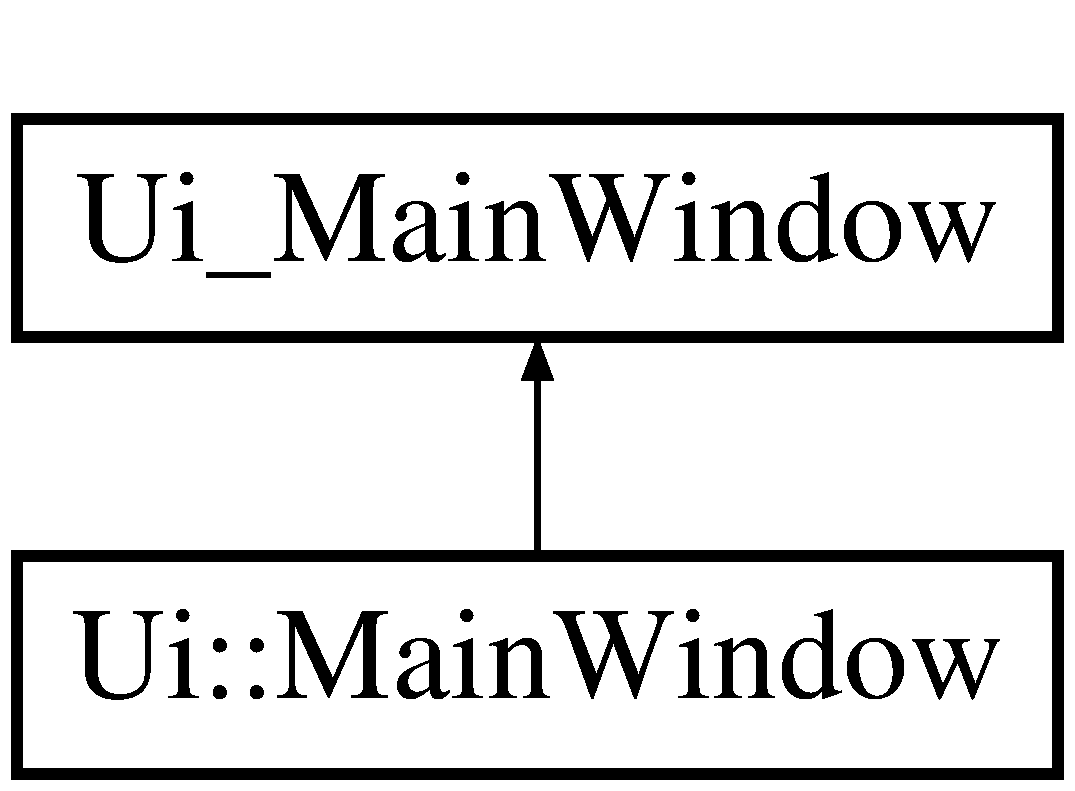
\includegraphics[height=2.000000cm]{class_ui___main_window}
\end{center}
\end{figure}
\subsection*{Public Member Functions}
\begin{DoxyCompactItemize}
\item 
\mbox{\Hypertarget{class_ui___main_window_acf4a0872c4c77d8f43a2ec66ed849b58}\label{class_ui___main_window_acf4a0872c4c77d8f43a2ec66ed849b58}} 
void {\bfseries setup\+Ui} (Q\+Main\+Window $\ast$\mbox{\hyperlink{class_main_window}{Main\+Window}})
\item 
\mbox{\Hypertarget{class_ui___main_window_a097dd160c3534a204904cb374412c618}\label{class_ui___main_window_a097dd160c3534a204904cb374412c618}} 
void {\bfseries retranslate\+Ui} (Q\+Main\+Window $\ast$\mbox{\hyperlink{class_main_window}{Main\+Window}})
\end{DoxyCompactItemize}
\subsection*{Public Attributes}
\begin{DoxyCompactItemize}
\item 
\mbox{\Hypertarget{class_ui___main_window_a30075506c2116c3ed4ff25e07ae75f81}\label{class_ui___main_window_a30075506c2116c3ed4ff25e07ae75f81}} 
Q\+Widget $\ast$ {\bfseries central\+Widget}
\item 
\mbox{\Hypertarget{class_ui___main_window_a40109d34201b8ce0fe88bfcf2e56132c}\label{class_ui___main_window_a40109d34201b8ce0fe88bfcf2e56132c}} 
Q\+Stacked\+Widget $\ast$ {\bfseries main\+\_\+stacked\+\_\+widget}
\item 
\mbox{\Hypertarget{class_ui___main_window_a8e4a8ffa90ddd4d78904fa36224ca803}\label{class_ui___main_window_a8e4a8ffa90ddd4d78904fa36224ca803}} 
Q\+Widget $\ast$ {\bfseries welcome\+\_\+page}
\item 
\mbox{\Hypertarget{class_ui___main_window_a58a84cd3057ab5459819f986b08942b1}\label{class_ui___main_window_a58a84cd3057ab5459819f986b08942b1}} 
Q\+Push\+Button $\ast$ {\bfseries start\+Button}
\item 
\mbox{\Hypertarget{class_ui___main_window_a4b5f6bad4de9498da2347576375c85e5}\label{class_ui___main_window_a4b5f6bad4de9498da2347576375c85e5}} 
Q\+Label $\ast$ {\bfseries welcome\+\_\+label}
\item 
\mbox{\Hypertarget{class_ui___main_window_a3c7da08ee61ff46bbf09a4adca920abb}\label{class_ui___main_window_a3c7da08ee61ff46bbf09a4adca920abb}} 
Q\+Label $\ast$ {\bfseries splash\+\_\+background}
\item 
\mbox{\Hypertarget{class_ui___main_window_ad9b9feb723ff2f77feaf7baf581f493c}\label{class_ui___main_window_ad9b9feb723ff2f77feaf7baf581f493c}} 
Q\+Label $\ast$ {\bfseries transparent\+\_\+box}
\item 
\mbox{\Hypertarget{class_ui___main_window_a9d2152dcebcac8e194ab28b061ba8121}\label{class_ui___main_window_a9d2152dcebcac8e194ab28b061ba8121}} 
Q\+Label $\ast$ {\bfseries transparent\+\_\+box\+\_\+2}
\item 
\mbox{\Hypertarget{class_ui___main_window_af4dccd8fafaacd32cfb5628a5f0dd951}\label{class_ui___main_window_af4dccd8fafaacd32cfb5628a5f0dd951}} 
Q\+Push\+Button $\ast$ {\bfseries A\+S\+U\+\_\+trip\+\_\+button}
\item 
\mbox{\Hypertarget{class_ui___main_window_aadb1a0d290c8d63116bcdf62d9f17438}\label{class_ui___main_window_aadb1a0d290c8d63116bcdf62d9f17438}} 
Q\+Push\+Button $\ast$ {\bfseries shortest\+\_\+trip\+\_\+button}
\item 
\mbox{\Hypertarget{class_ui___main_window_a4c26d9d636b74280530ccc221bc1e820}\label{class_ui___main_window_a4c26d9d636b74280530ccc221bc1e820}} 
Q\+Widget $\ast$ {\bfseries tours\+\_\+page}
\item 
\mbox{\Hypertarget{class_ui___main_window_a08a857edea57a9e53915f22187c06813}\label{class_ui___main_window_a08a857edea57a9e53915f22187c06813}} 
Q\+Widget $\ast$ {\bfseries grid\+Layout\+Widget}
\item 
\mbox{\Hypertarget{class_ui___main_window_a525ed3c5fe0784ac502ee222fba4e205}\label{class_ui___main_window_a525ed3c5fe0784ac502ee222fba4e205}} 
Q\+Grid\+Layout $\ast$ {\bfseries grid\+Layout}
\item 
\mbox{\Hypertarget{class_ui___main_window_a09729e39800ff7505526d04733e908ed}\label{class_ui___main_window_a09729e39800ff7505526d04733e908ed}} 
Q\+Label $\ast$ {\bfseries choosing\+\_\+label}
\item 
\mbox{\Hypertarget{class_ui___main_window_a4acc75016fe249ce9e6e7068c446fed2}\label{class_ui___main_window_a4acc75016fe249ce9e6e7068c446fed2}} 
Q\+Widget $\ast$ {\bfseries admin\+\_\+login\+\_\+page}
\item 
\mbox{\Hypertarget{class_ui___main_window_a2579954606928880d642aeb6b6881729}\label{class_ui___main_window_a2579954606928880d642aeb6b6881729}} 
Q\+Label $\ast$ {\bfseries transparent\+\_\+box\+\_\+3}
\item 
\mbox{\Hypertarget{class_ui___main_window_ae3d18455329e01d882a0ecad2d362b8d}\label{class_ui___main_window_ae3d18455329e01d882a0ecad2d362b8d}} 
Q\+Label $\ast$ {\bfseries error\+\_\+label}
\item 
\mbox{\Hypertarget{class_ui___main_window_a87406b092794f44a03c6d46e6e8ff3d7}\label{class_ui___main_window_a87406b092794f44a03c6d46e6e8ff3d7}} 
Q\+Push\+Button $\ast$ {\bfseries back\+\_\+button}
\item 
\mbox{\Hypertarget{class_ui___main_window_af8bd562e97560e62ab5d92175562eb03}\label{class_ui___main_window_af8bd562e97560e62ab5d92175562eb03}} 
Q\+Push\+Button $\ast$ {\bfseries login\+\_\+button}
\item 
\mbox{\Hypertarget{class_ui___main_window_a15377a17a988ecff22d07151512739b0}\label{class_ui___main_window_a15377a17a988ecff22d07151512739b0}} 
Q\+Line\+Edit $\ast$ {\bfseries password\+\_\+line\+\_\+edit}
\item 
\mbox{\Hypertarget{class_ui___main_window_a22f01013c85d5a0814c165672a5d7a72}\label{class_ui___main_window_a22f01013c85d5a0814c165672a5d7a72}} 
Q\+Line\+Edit $\ast$ {\bfseries username\+\_\+line\+\_\+edit}
\item 
\mbox{\Hypertarget{class_ui___main_window_aa18dcb4d8ddc02fcc88e3e60c5839aaf}\label{class_ui___main_window_aa18dcb4d8ddc02fcc88e3e60c5839aaf}} 
Q\+Label $\ast$ {\bfseries password\+\_\+label}
\item 
\mbox{\Hypertarget{class_ui___main_window_abe90689289a4045c990fbc37d1152c98}\label{class_ui___main_window_abe90689289a4045c990fbc37d1152c98}} 
Q\+Label $\ast$ {\bfseries username\+\_\+label}
\item 
\mbox{\Hypertarget{class_ui___main_window_a9a445d58453e8e234de066547143246e}\label{class_ui___main_window_a9a445d58453e8e234de066547143246e}} 
Q\+Label $\ast$ {\bfseries admin\+\_\+login\+\_\+label}
\item 
\mbox{\Hypertarget{class_ui___main_window_a27e0b134c3c12643afbf0b50dd175453}\label{class_ui___main_window_a27e0b134c3c12643afbf0b50dd175453}} 
Q\+Frame $\ast$ {\bfseries line\+\_\+3}
\item 
\mbox{\Hypertarget{class_ui___main_window_add492bf5763815e82fba9ba9297c50e6}\label{class_ui___main_window_add492bf5763815e82fba9ba9297c50e6}} 
Q\+Frame $\ast$ {\bfseries line\+\_\+4}
\item 
\mbox{\Hypertarget{class_ui___main_window_a7fd61d9f66189e10dcae1147f0a48e04}\label{class_ui___main_window_a7fd61d9f66189e10dcae1147f0a48e04}} 
Q\+Frame $\ast$ {\bfseries line\+\_\+5}
\item 
\mbox{\Hypertarget{class_ui___main_window_a6a831aebdb3e8e8b1d7ba144f013d3cd}\label{class_ui___main_window_a6a831aebdb3e8e8b1d7ba144f013d3cd}} 
Q\+Label $\ast$ {\bfseries maintenance\+\_\+label}
\item 
\mbox{\Hypertarget{class_ui___main_window_a20d3451b9fb457067a4874c5a221fc67}\label{class_ui___main_window_a20d3451b9fb457067a4874c5a221fc67}} 
Q\+Widget $\ast$ {\bfseries maintenance\+\_\+page}
\item 
\mbox{\Hypertarget{class_ui___main_window_a85167df8895285b886db755d66ab53d8}\label{class_ui___main_window_a85167df8895285b886db755d66ab53d8}} 
Q\+List\+Widget $\ast$ {\bfseries souvenir\+\_\+list\+\_\+widget}
\item 
\mbox{\Hypertarget{class_ui___main_window_a16e802a7ebd4beb9d8aba858565e51b3}\label{class_ui___main_window_a16e802a7ebd4beb9d8aba858565e51b3}} 
Q\+Frame $\ast$ {\bfseries line}
\item 
\mbox{\Hypertarget{class_ui___main_window_af363d01e21581b1df12446fef60aac8b}\label{class_ui___main_window_af363d01e21581b1df12446fef60aac8b}} 
Q\+Push\+Button $\ast$ {\bfseries exit\+\_\+button}
\item 
\mbox{\Hypertarget{class_ui___main_window_a17207206e55a605ecc14a3534b7e575f}\label{class_ui___main_window_a17207206e55a605ecc14a3534b7e575f}} 
Q\+Frame $\ast$ {\bfseries line\+\_\+2}
\item 
\mbox{\Hypertarget{class_ui___main_window_ad01968740c435709a8b2ec4c08094c67}\label{class_ui___main_window_ad01968740c435709a8b2ec4c08094c67}} 
Q\+Frame $\ast$ {\bfseries frame}
\item 
\mbox{\Hypertarget{class_ui___main_window_a6b2a0c5f7e8ff2a87134908dd770d2d2}\label{class_ui___main_window_a6b2a0c5f7e8ff2a87134908dd770d2d2}} 
Q\+Grid\+Layout $\ast$ {\bfseries grid\+Layout\+\_\+2}
\item 
\mbox{\Hypertarget{class_ui___main_window_af13749cb2b165e2f3ba8b7bd00b147f0}\label{class_ui___main_window_af13749cb2b165e2f3ba8b7bd00b147f0}} 
Q\+Push\+Button $\ast$ {\bfseries add\+\_\+souvenir\+\_\+button}
\item 
\mbox{\Hypertarget{class_ui___main_window_a6070a3cacbf1c312b60b98890956793a}\label{class_ui___main_window_a6070a3cacbf1c312b60b98890956793a}} 
Q\+Push\+Button $\ast$ {\bfseries upload\+\_\+college\+\_\+button}
\item 
\mbox{\Hypertarget{class_ui___main_window_ac9787d5b5c982f33216bba1199894d68}\label{class_ui___main_window_ac9787d5b5c982f33216bba1199894d68}} 
Q\+Label $\ast$ {\bfseries header\+\_\+label}
\item 
\mbox{\Hypertarget{class_ui___main_window_a90431db020b6a6b931d7170a538c8002}\label{class_ui___main_window_a90431db020b6a6b931d7170a538c8002}} 
Q\+Push\+Button $\ast$ {\bfseries header\+\_\+icon\+\_\+push\+\_\+button}
\item 
\mbox{\Hypertarget{class_ui___main_window_a7835addb33294b225483cf76825365a8}\label{class_ui___main_window_a7835addb33294b225483cf76825365a8}} 
Q\+Push\+Button $\ast$ {\bfseries admin\+\_\+push\+\_\+button}
\item 
\mbox{\Hypertarget{class_ui___main_window_aef012e34567cf1c9317a2560adef17b5}\label{class_ui___main_window_aef012e34567cf1c9317a2560adef17b5}} 
Q\+Label $\ast$ {\bfseries admin\+\_\+label}
\item 
\mbox{\Hypertarget{class_ui___main_window_a3039ec67b5f2d9e4e0e30f1f94323690}\label{class_ui___main_window_a3039ec67b5f2d9e4e0e30f1f94323690}} 
Q\+Frame $\ast$ {\bfseries header\+\_\+line}
\item 
\mbox{\Hypertarget{class_ui___main_window_ab96ab0f0578098521fa69a75aa5cdde8}\label{class_ui___main_window_ab96ab0f0578098521fa69a75aa5cdde8}} 
Q\+Widget $\ast$ {\bfseries layout\+Widget}
\item 
\mbox{\Hypertarget{class_ui___main_window_afedcce3d8f3dddf4c1fd5b768660b8ee}\label{class_ui___main_window_afedcce3d8f3dddf4c1fd5b768660b8ee}} 
Q\+Form\+Layout $\ast$ {\bfseries form\+Layout}
\item 
\mbox{\Hypertarget{class_ui___main_window_aab31b3dec8d767525dea6f163e029e48}\label{class_ui___main_window_aab31b3dec8d767525dea6f163e029e48}} 
Q\+Widget $\ast$ {\bfseries layout\+Widget1}
\item 
\mbox{\Hypertarget{class_ui___main_window_adb9e9053924d82773ec4e07e6c96271f}\label{class_ui___main_window_adb9e9053924d82773ec4e07e6c96271f}} 
Q\+Form\+Layout $\ast$ {\bfseries form\+Layout\+\_\+2}
\item 
\mbox{\Hypertarget{class_ui___main_window_a2be1c24ec9adfca18e1dcc951931457f}\label{class_ui___main_window_a2be1c24ec9adfca18e1dcc951931457f}} 
Q\+Menu\+Bar $\ast$ {\bfseries menu\+Bar}
\item 
\mbox{\Hypertarget{class_ui___main_window_a5172877001c8c7b4e0f6de50421867d1}\label{class_ui___main_window_a5172877001c8c7b4e0f6de50421867d1}} 
Q\+Tool\+Bar $\ast$ {\bfseries main\+Tool\+Bar}
\item 
\mbox{\Hypertarget{class_ui___main_window_a50fa481337604bcc8bf68de18ab16ecd}\label{class_ui___main_window_a50fa481337604bcc8bf68de18ab16ecd}} 
Q\+Status\+Bar $\ast$ {\bfseries status\+Bar}
\end{DoxyCompactItemize}


The documentation for this class was generated from the following file\+:\begin{DoxyCompactItemize}
\item 
ui\+\_\+mainwindow.\+h\end{DoxyCompactItemize}

\hypertarget{class_ui__totals}{}\section{Ui\+\_\+totals Class Reference}
\label{class_ui__totals}\index{Ui\+\_\+totals@{Ui\+\_\+totals}}
Inheritance diagram for Ui\+\_\+totals\+:\begin{figure}[H]
\begin{center}
\leavevmode
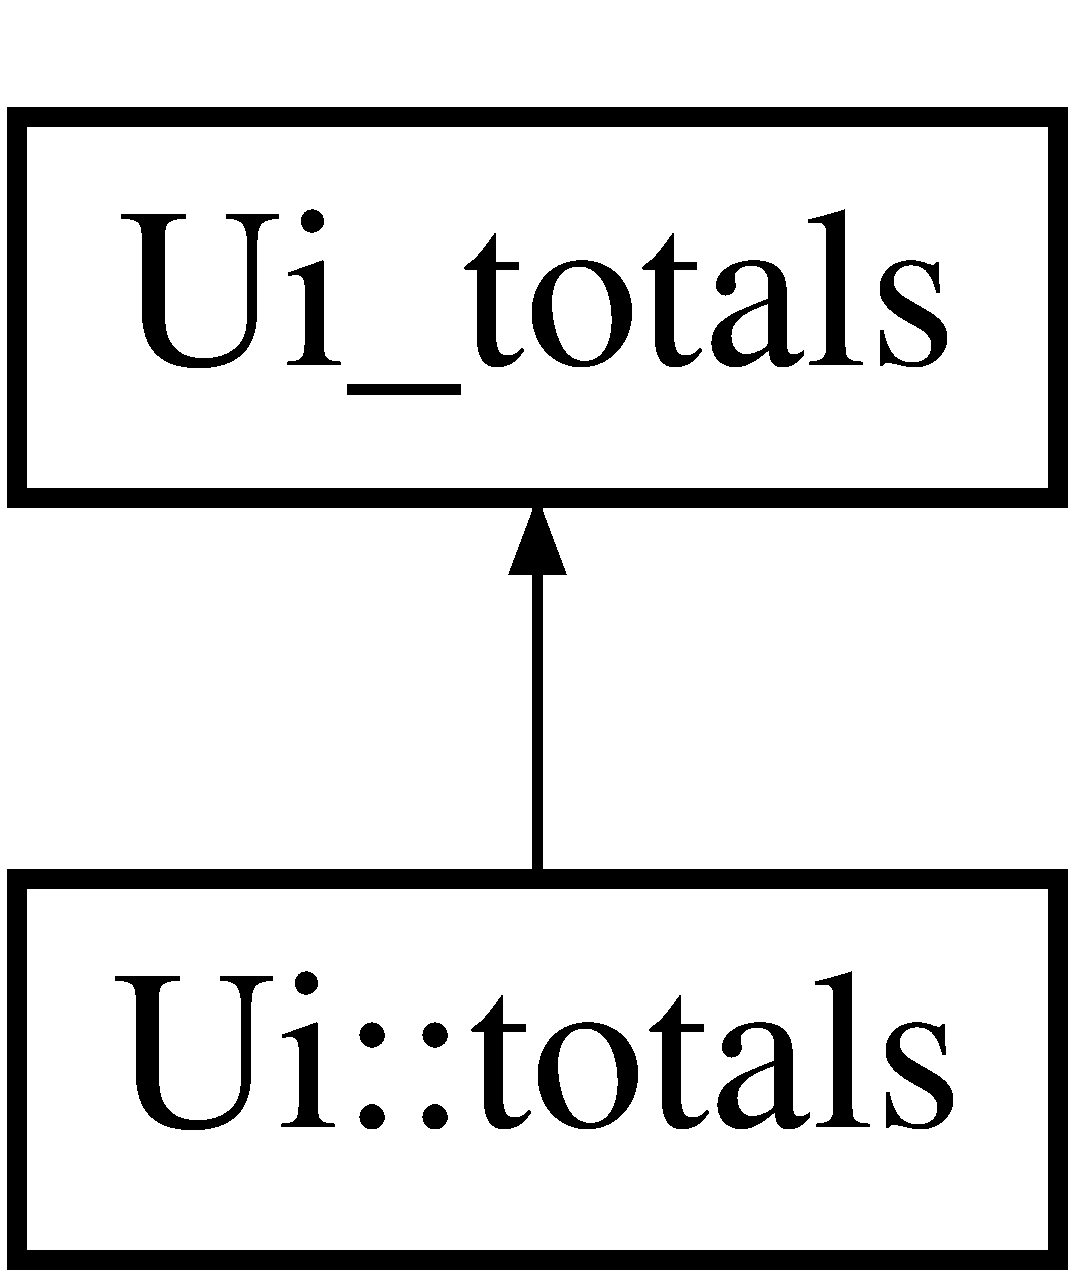
\includegraphics[height=2.000000cm]{class_ui__totals}
\end{center}
\end{figure}
\subsection*{Public Member Functions}
\begin{DoxyCompactItemize}
\item 
\mbox{\Hypertarget{class_ui__totals_a7340762e897871f4d67313ca67644bbe}\label{class_ui__totals_a7340762e897871f4d67313ca67644bbe}} 
void {\bfseries setup\+Ui} (Q\+Widget $\ast$totals)
\item 
\mbox{\Hypertarget{class_ui__totals_a903318c2f0c546b0ab49a8ec95e6d3aa}\label{class_ui__totals_a903318c2f0c546b0ab49a8ec95e6d3aa}} 
void {\bfseries retranslate\+Ui} (Q\+Widget $\ast$totals)
\end{DoxyCompactItemize}
\subsection*{Public Attributes}
\begin{DoxyCompactItemize}
\item 
\mbox{\Hypertarget{class_ui__totals_a57aeecd124fbac456c83be9bca8f603d}\label{class_ui__totals_a57aeecd124fbac456c83be9bca8f603d}} 
Q\+List\+Widget $\ast$ {\bfseries totals\+\_\+list}
\end{DoxyCompactItemize}


The documentation for this class was generated from the following file\+:\begin{DoxyCompactItemize}
\item 
ui\+\_\+totals.\+h\end{DoxyCompactItemize}

\hypertarget{class_ui__totals_sheet}{}\section{Ui\+\_\+totals\+Sheet Class Reference}
\label{class_ui__totals_sheet}\index{Ui\+\_\+totals\+Sheet@{Ui\+\_\+totals\+Sheet}}
Inheritance diagram for Ui\+\_\+totals\+Sheet\+:\begin{figure}[H]
\begin{center}
\leavevmode
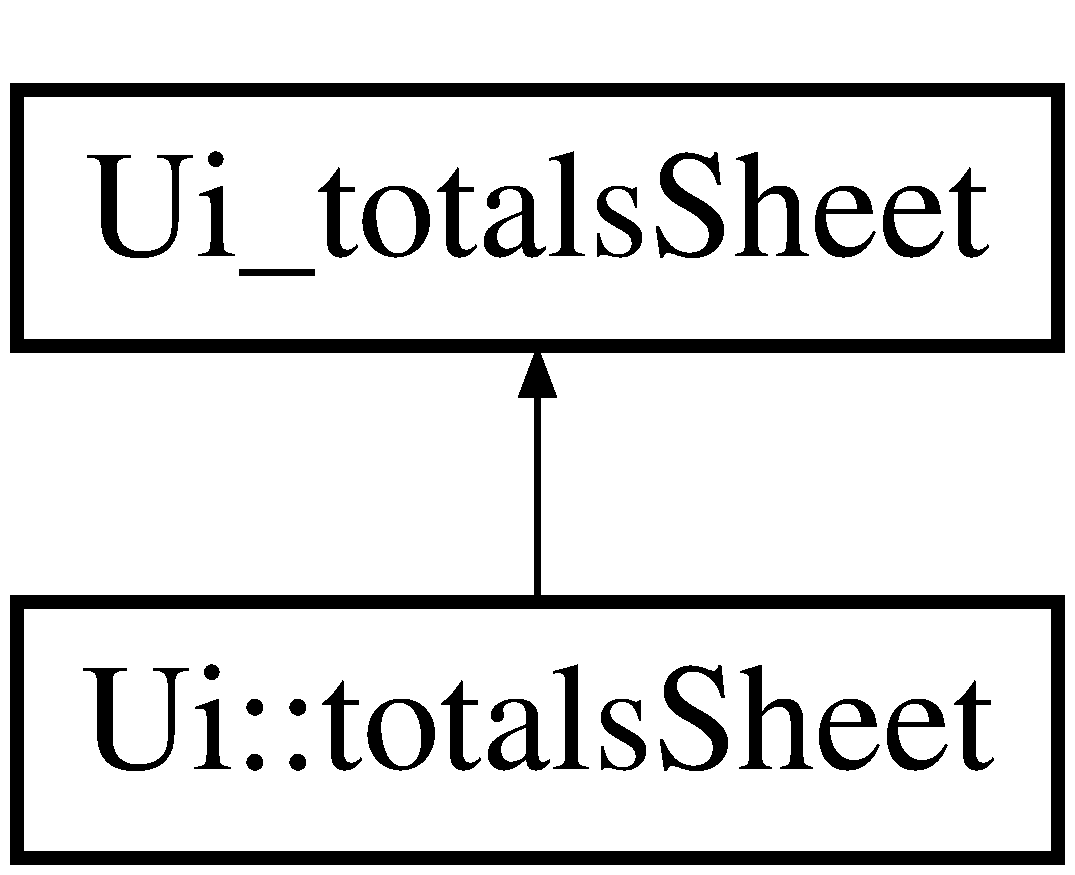
\includegraphics[height=2.000000cm]{class_ui__totals_sheet}
\end{center}
\end{figure}
\subsection*{Public Member Functions}
\begin{DoxyCompactItemize}
\item 
\mbox{\Hypertarget{class_ui__totals_sheet_a90335aca2c8a8a84d29cc992eeaa3988}\label{class_ui__totals_sheet_a90335aca2c8a8a84d29cc992eeaa3988}} 
void {\bfseries setup\+Ui} (Q\+Dialog $\ast$\mbox{\hyperlink{classtotals_sheet}{totals\+Sheet}})
\item 
\mbox{\Hypertarget{class_ui__totals_sheet_ad75f938fe32afcef82d47226c1d021cc}\label{class_ui__totals_sheet_ad75f938fe32afcef82d47226c1d021cc}} 
void {\bfseries retranslate\+Ui} (Q\+Dialog $\ast$\mbox{\hyperlink{classtotals_sheet}{totals\+Sheet}})
\end{DoxyCompactItemize}
\subsection*{Public Attributes}
\begin{DoxyCompactItemize}
\item 
\mbox{\Hypertarget{class_ui__totals_sheet_a845593c67f994a3552591122a1b28b87}\label{class_ui__totals_sheet_a845593c67f994a3552591122a1b28b87}} 
Q\+Grid\+Layout $\ast$ {\bfseries grid\+Layout}
\item 
\mbox{\Hypertarget{class_ui__totals_sheet_a6ac7b4641e346339038e830fc255c014}\label{class_ui__totals_sheet_a6ac7b4641e346339038e830fc255c014}} 
Q\+List\+Widget $\ast$ {\bfseries totals\+\_\+list}
\end{DoxyCompactItemize}


The documentation for this class was generated from the following file\+:\begin{DoxyCompactItemize}
\item 
ui\+\_\+totalssheet.\+h\end{DoxyCompactItemize}

%--- End generated contents ---

% Index
\backmatter
\newpage
\phantomsection
\clearemptydoublepage
\addcontentsline{toc}{chapter}{Index}
\printindex

\end{document}
